%% !TeX program = LuaLaTeX
%% !TeX encoding = UTF-8

%----------------------------------------------------------------------------------------
%	PACKAGES AND OTHER DOCUMENT CONFIGURATIONS
%----------------------------------------------------------------------------------------
%\UseRawInputEncoding
%\DeclareUnicodeCharacter{00A0}{~}
\documentclass[ 
11pt, % The default document font size, options: 10pt, 11pt, 12pt
% oneside, % Two side (alternating margins) for binding by default, uncomment to switch to one side
french, % ngerman for German
singlespacing, % Single line spacing, alternatives: onehalfspacing or doublespacing
% draft, % Uncomment to enable draft mode (no pictures, no links, overfull hboxes indicated)
%nolistspacing, % If the document is onehalfspacing or doublespacing, uncomment this to set spacing in lists to single
% liststotoc, % Uncomment to add the list of figures/tables/etc to the table of contents
%toctotoc, % Uncomment to add the main table of contents to the table of contents
parskip, % Uncomment to add space between paragraphs
%nohyperref, % Uncomment to not load the hyperref package
headsepline, % Uncomment to get a line under the header
%chapterinoneline, % Uncomment to place the chapter title next to the number on one line
%consistentlayout, % Uncomment to change the layout of the declaration, abstract and acknowledgements pages to match the default layout
openany, %% Use this option to make chapters start on the next page, irrespective of whether it's an odd or even numbered page
]{MastersDoctoralThesis} % The class file specifying the document structure

% \usepackage{mathpazo} % Use the Palatino font by default
% \usepackage[charter]{mathdesign}

\usepackage{kpfonts}        %% For math only
\usepackage{fontspec}       %% Because we are using XeTEX
\setromanfont{Minion Pro}   %% For text (Minion Math is commercial)



% \setcounter{tocdepth}{4} %% Use this to set numbering depth for sections in the toc (already set in the Class)
\setcounter{secnumdepth}{3} %% Use this to set numbering depth for sections in the whole document

\graphicspath{ {./Figures/} } %% To load all images in this document from the Figures directory
\DeclareGraphicsExtensions{.pdf,.png}  %% Use to this to set the priority for extensions leading
\usepackage[font=sf,labelfont=bf]{caption}
\usepackage[font=sf]{floatrow}  %% For other floet content
% \captionsetup[figure]{font=it}
\usepackage{subcaption} %% Use to make subgraphics
\usepackage{float} %% Use this to control where the images are placed compared to thier related text
\usepackage{multirow}

\usepackage{tikz}
\usetikzlibrary{patterns}
\usepackage{tikzscale}

%\usepackage{amssymb}
%\usepackage{amsthm}
\usepackage{amsmath,bm,mathtools} %% Use this to include the "align" environment in witch equations can be made easier
\usepackage{physics} %% To have physical terms like the divergence operator

%\usepackage[backend=bibtex,style=numeric,maxnames=2,natbib=true]{biblatex} % Use the bibtex backend with the numeric citation style
\usepackage[backend=bibtex,style=alphabetic,maxnames=2,natbib=true]{biblatex} % Use the bibtex backend with the authoryear citation style (which resembles APA)
% \bibliographystyle{abbrv}
%\usepackage[backend=bibtex,style=authoryear-comp,sorting=none,sortcites=true,doi=false,url=false,giveninits=true,hyperref]{biblatex}

\addbibresource{bibliography.bib} % The filename of the bibliography
\addbibresource{bibliography_matthias.bib} % The filename of the bibliography

\usepackage[autostyle=true]{csquotes} % Required to generate language-dependent quotes in the bibliography 

\usepackage{indentfirst}  %% For indentation

\usepackage{xcolor}   %% To add color to text

\usepackage{hyperref}
\usepackage{cleveref} %% To reference stuf
\usepackage{upgreek}

%----------------------------------------------------------------------------------------

\renewcommand{\emph}[1]{\textbf{\textit{#1}}} %% Use this to make \emph text bold (you lose all other properties of the command)

\newcommand{\Run}{\mathbb{R}}
\newcommand{\Rdeux}{\mathbb{R}^2}
\newcommand{\Rtrois}{\mathbb{R}^3}
\newcommand{\hplus}{h_{+}}
\newcommand{\hmoins}{h_{-}}
\newcommand{\eun}{\bvec{e}_1(\omega)}
\newcommand{\edeux}{\bvec{e}_2(\omega)}

\newcommand{\bvec}[1]{\bm{\mathrm{#1}}}  %% Use this to make vectors
\newcommand{\bmat}[1]{\bm{\mathsf{#1}}}   %% Use this to make tensors

\newcommand{\R}{\mathcal{R}}
\renewcommand{\P}{\mathcal{P}}

\newcommand{\diff}{\,\differential}
\newcommand{\intO}[1]{\int_{\Omega^{#1}(t)}}
\newcommand{\dtstar}{\delta t^*}

\newcommand{\identity}{\text{Id}}

\newcommand{\eel}{E_{\text{el}}}
\newcommand{\efrac}{E_{\text{frac}}}
\newcommand{\etot}{E_{\text{tot}}}
\newcommand{\wadm}{W_{\text{adm}}}

\newtheorem{theorem}{Theorem}
\numberwithin{theorem}{section}  %% Pour numeroter par section

%----------------------------------------------------------------------------------------
%	MARGIN SETTINGS
%----------------------------------------------------------------------------------------

%% To have a uniform margin on all pages
\geometry{
	paper=a4paper, % Change to letterpaper for US letter
	inner=0.75in, % Inner margin
	outer=0.75in, % Outer margin
	bindingoffset=.5cm, % Binding offset
	top=1.5cm, % Top margin
	bottom=1.5cm, % Bottom margin
	%showframe, % Uncomment to show how the type block is set on the page
}

%----------------------------------------------------------------------------------------
%	THESIS INFORMATION
%----------------------------------------------------------------------------------------

\thesistitle{Fracturation de floes de glace par percussion dans un modèle granulaire} % Your thesis title, ths is used in the title and abstract, print it elsewhere with \ttitle
\supervisor{\href{http://mduprez.perso.math.cnrs.fr/}{Stéphane \textsc{Labbé}}} % Your supervisor's name, this is used in the title page, print it elsewhere with \supname
\examiner{Christophe \textsc{Prud'homme}} % Your examiner's name, this is not currently used anywhere in the template, print it elsewhere with \examname
\degree{master 2 CSMI} % Your degree name, this is used in the title page and abstract, print it elsewhere with \degreename
\author{Roussel Desmond \textsc{Nzoyem}} % Your name, this is used in the title page and abstract, print it elsewhere with \authorname
\addresses{} % Your address, this is not currently used anywhere in the template, print it elsewhere with \addressname

\subject{Mathématiques appliquées} % Your subject area, this is not currently used anywhere in the template, print it elsewhere with \subjectname
\keywords{} % Keywords for your thesis, this is not currently used anywhere in the template, print it elsewhere with \keywordnames
\university{\href{http://www.unistra.fr}{University of Strasbourg, Sorbonne Unisersité}} % Your university's name and URL, this is used in the title page and abstract, print it elsewhere with \univname
\department{\href{https://mathinfo.unistra.fr/}{UFR de mathématiques et d'informatique}} % Your department's name and URL, this is used in the title page and abstract, print it elsewhere with \deptname
\group{\href{https://mimesis.inria.fr/}{SASIP}} % Your research group's name and URL, this is used in the title page, print it elsewhere with \groupname
\faculty{\href{https://mathinfo.unistra.fr/}{UFR de mathématiques et d'informatique}} % Your faculty's name and URL, this is used in the title page and abstract, print it elsewhere with \facname

\AtBeginDocument{
\hypersetup{pdftitle=\ttitle} % Set the PDF's title to your title
\hypersetup{pdfauthor=\authorname} % Set the PDF's author to your name
\hypersetup{pdfkeywords=\keywordnames} % Set the PDF's keywords to your keywords
}


%\pdfmapfile{=/var/lib/texmf/fonts/map/pdftex/updmap/pdftex.map}

\begin{document}

\frontmatter % Use roman page numbering style (i, ii, iii, iv...) for the pre-content pages

\pagestyle{plain} % Default to the plain heading style until the thesis style is called for the body content

%----------------------------------------------------------------------------------------
%	TITLE PAGE
%----------------------------------------------------------------------------------------

\begin{titlepage}

\begin{figure}[!htb]
   \begin{minipage}{0.32\textwidth}
     \centering
     \vspace*{12pt}
     \includegraphics[width=.8\linewidth]{LogoUnistra2.png}
     \label{Fig:LogoUnistra}
   \end{minipage}\hspace*{7pt}
   \begin{minipage}{0.32\textwidth}
    \centering
    \includegraphics[width=.5\linewidth]{LogoLJLL.jpg}
    \label{Fig:LogoMimesis}
  \end{minipage}\hfill
   \begin{minipage}{0.32\textwidth}
     \centering
     \includegraphics[width=.8\linewidth]{LogoCSMI.png}
     \label{Fig:LogoInria}
   \end{minipage}
\end{figure}


\begin{center}

\vspace*{.04\textheight}
% {\scshape\LARGE \univname\par}\vspace{1.5cm} % University name
\textsc{\Large Rapport de stage}\\[0.5cm] % Thesis type

\HRule \\[0.4cm] % Horizontal line
{\huge \bfseries \ttitle\par}\vspace{0.4cm} % Thesis title
\HRule \\[1.5cm] % Horizontal line

\begin{minipage}[t]{0.4\textwidth}
\begin{flushleft} \large
\vspace{7mm}
\emph{Étudiant}\\
\href{https://github.com/desmond-rn}{\authorname} % Author name - remove the \href bracket to remove the link
\end{flushleft}
\end{minipage}
\begin{minipage}[t]{0.4\textwidth}
\begin{flushright} \large
\emph{Superviseur} \\
\href{http://mduprez.perso.math.cnrs.fr/}{\supname} % Supervisor names - remove the \href bracket to remove the link
\\ \vspace{5mm}
\emph{Enseignant référent} \\
\href{http://www.feelpp.org/team/prudhomm/}{\examname} % Examiner's name - remove the \href bracket to remove the link
\end{flushright}
\end{minipage}%%\\[2cm]

% \vfill

\begin{figure}[H]
    \centering
    \includegraphics[width=.9\linewidth]{IntroPic.jpg}
    \label{Fig:IntroPic}
\end{figure}


\large \textit{Ce stage à été effectué dans le cadre du \href{https://docs.google.com/document/d/10JbbXeqqu5J2BjMkSQRNQ8Gx7xBPOClLKpvd7EBZT8U/edit}{master 2 CSMI,}}\\[0.2cm]
\textit{du 03 février 2021, au 31 juillet 2021;}\\[0.2cm]
\textit{initié par le groupe \groupname \hspace*{1pt} au \href{https://www.ljll.math.upmc.fr/?lang=fr}{LJLL}.}\\[0.2cm]

\vspace*{.04\textheight}
\large Année académique 2020 - 2021

\vfill

{\large \today}\\[4cm] % Today's date
% \includegraphics{Logo_UNIV} % University/department logo - uncomment to place it

% \vfill
\end{center}
\end{titlepage}

%----------------------------------------------------------------------------------------
%	DECLARATION PAGE
%----------------------------------------------------------------------------------------
%
% \begin{declaration}  
% \addchaptertocentry{\authorshipname} % Add the declaration to the table of contents
% \not I, \authorname, declare that this thesis titled, \enquote{\ttitle} and the work presented in it are my own. I confirm that:
%
% \begin{itemize}
% \item This work was done wholly or mainly while in candidature for a research degree at this University.
% \item Where any part of this thesis has previously been submitted for a degree or any other qualification at this University or any other institution, this has been clearly stated.
% \item Where I have consulted the published work of others, this is always clearly attributed.
% \item Where I have quoted from the work of others, the source is always given. With the exception of such quotations, this thesis is entirely my own work.
% \item I have acknowledged all main sources of help.
% \item Where the thesis is based on work done by myself jointly with others, I have made clear exactly what was done by others and what I have contributed myself.\\
% \end{itemize}
%
% \noindent Signed:\\
% \rule[0.5em]{25em}{0.5pt} % This prints a line for the signature
%
% \noindent Date:\\
% \rule[0.5em]{25em}{0.5pt} % This prints a line to write the date
% \end{declaration}
%
% \cleardoublepage

%----------------------------------------------------------------------------------------
%	QUOTATION PAGE
%----------------------------------------------------------------------------------------
%
% \vspace*{0.2\textheight}
%
% \noindent\enquote{\itshape Thanks to my solid academic training, today I can write hundreds of words on virtually any topic without possessing a shred of information, which is how I got a good job in journalism.}\bigbreak
%
% \hfill Dave Barry

%----------------------------------------------------------------------------------------
%	ABSTRACT PAGE
%----------------------------------------------------------------------------------------
%
% \begin{abstract}
% \addchaptertocentry{\abstractname} % Add the abstract to the table of contents
% The Thesis Abstract is written here (and usually kept to just this page). The page is kept centered vertically so can expand into the blank space above the title too\ldots
% \end{abstract}

% ----------------------------------------------------------------------------------------
% 	ACKNOWLEDGEMENTS
% ----------------------------------------------------------------------------------------

\begin{acknowledgements}
\addchaptertocentry{\acknowledgementname} % Add the acknowledgements to the table of contents

\end{acknowledgements}

%----------------------------------------------------------------------------------------
%	LIST OF CONTENTS/FIGURES/TABLES PAGES
%----------------------------------------------------------------------------------------

\tableofcontents % Prints the main table of contents

% \listoffigures % Prints the list of figures

% \listoftables % Prints the list of tables

%----------------------------------------------------------------------------------------
%	ABBREVIATIONS
%----------------------------------------------------------------------------------------

% \begin{abbreviations}{11} % Include a list of abbreviations (a table of two columns)
% 
% \addchaptertocentry{\abbreviations} % Add the abbreviations to the table of contents
% \textbf{ETR} & \textbf{E}quation (du) \textbf{T}ransfert \textbf{R}adiatif\\
% \textbf{ETL} & \textbf{E}quilibre \textbf{T}hermique \textbf{L}ocal\\
% \textbf{UFR} & \textbf{U}nite de\textbf{F}ormation et de \textbf{R}echerche de l'Universite de Strasbourg
% 
% \end{abbreviations}

%----------------------------------------------------------------------------------------
%	PHYSICAL CONSTANTS/OTHER DEFINITIONS
%----------------------------------------------------------------------------------------

% \begin{constants}{lr@{${}={}$}l} % The list of physical constants is a three column table
% 
% The \SI{}{} command is provided by the siunitx package, see its documentation for instructions on how to use it
% 
% Speed of Light & $c_{0}$ & \SI{2.99792458e8}{\meter\per\second} (exact)\\
% Constant Name & $Symbol$ & $Constant Value$ with units\\

% \end{constants}

%----------------------------------------------------------------------------------------
%	SYMBOLS
%----------------------------------------------------------------------------------------

% \begin{symbols}{rcc} % Include a list of Symbols (a three column table)
% \label{sec:symbols}
% \textbf{Symbole} & \textbf{Définition} & \textbf{Unité} \\
% \addlinespace % Gap to separate the Roman symbols from the Greek

% $x$ & Abscisse & \si{\cm} \\
% $y$ & Ordonnée & \si{\cm} \\
% $\bvec{x}$ & Vecteur position & \si{\cm} \\
% $\bm{\Omega}$ & Vecteur direction de propagation des photons & \si{\cm^2 \per \cm^2} \\
% $\nu$ & Fréquence & \si{Hz} \\
% $p$ & Fonction de distribution angulaire de « scattering » &  \\
% $I$ & Intensité spécifique de radiation & \si{W \per m^2 \per sr  \per Hz} \\
% $B$ & Fonction de Planck & \si{W \per m^2 \per sr  \per Hz} \\

% \addlinespace % Gap with real SI dimensions

% $\rho$ & Densité du milieu & \si{\g \per \cm\cubed} \\
% $\sigma_a$ & Opacité d'absorption & \si{\per\cm} \\
% $\sigma_c$ & Opacité de « scattering » (ou de dispersion) & \si{\per\cm} \\

% \addlinespace % Gap to separate inputs

% $t$ & Temps & \si{sh} \\
% $C_v$ & Capacité thermique du milieu & \si{Jerk \per\g \per keV} \\
% $a$ & Constante radiative (ou de rayonnement)& \si{g \per cm \per sh^2  \per keV } \\
% $c$ & Vitesse de la lumière & \si{\cm \per sh} \\

% \addlinespace % Gap to separate output

% $T$ & Température matière & \si{keV} \\
% $E$ & Energie des photons & \si{g \per \cm \per sh^2} \\
% $\bvec{F}$ & Flux de photons & \si{g \per sh^2} \\

% \end{symbols}

%----------------------------------------------------------------------------------------
%	DEDICATION
%----------------------------------------------------------------------------------------

% \dedicatory{For/Dedicated to/To my\ldots}

%----------------------------------------------------------------------------------------
%	THESIS CONTENT - CHAPTERS
%----------------------------------------------------------------------------------------

\mainmatter % Begin numeric (1,2,3...) page numbering
\setlength{\parindent}{4ex} %% Set the paragraph indentation as from this line

\pagestyle{thesis} % Return the page headers back to the "thesis" style

% Include the chapters of the thesis as separate files from the Chapters folder
% Uncomment the lines as you write the chapters

% % Chapter 1

\chapter{Introduction} % Main chapter title

\label{Chapter1} % For referencing the chapter elsewhere, use \ref{Chapter1} 

%----------------------------------------------------------------------------------------

% Define some commands to keep the formatting separated from the content 
\newcommand{\keyword}[1]{\textbf{#1}}
\newcommand{\tabhead}[1]{\textbf{#1}}
\newcommand{\code}[1]{\texttt{#1}}
\newcommand{\file}[1]{\texttt{\bfseries#1}}
\newcommand{\option}[1]{\texttt{\itshape#1}}






%1----------------------------------------------------------------------------------------



\section{Contexte}



Le déclin de la glace Artique ces dernières décenies est considéré comme l'une manifestations les plus marquante du changement climatique (voir \parencite{stroeve2012trends}). Ce déclin présente des enjeux aussi climatiques qu'industriels. Premièrement, de par son étendue et son epaisseur immense, la la zone artique est un contributeur majeur climat à travers ses échanges de chaleurs par rayonnement et radiation avec l'atmosphère. Il est donc crucial de considérer l'évolution de la glace dans les modèles climatiques. Deuxièmement, la chute de cette couverture de glace dans la MIZ\footnote{Marginal Ice Zone : zone de transition entre l’océan et le coeur de la banquise, où la concentration de
glace est inférieure à 80\%, et/ou les morceaux de glace sont de faible épaisseur ($\approx 1 mètre$) et de petite taille ($10 m - 100 km$).} (VOIR FIGURE) ouvre des routes maritimes facilitant l'exploitation de ses réserves d’hydrocarbures (qui restent quasiment intactes). Il est donc nécéssaire de pouvoir prédire l'évolution de la banquise Artique (au moins) à court terme.


Parmis les élément exhaxerbant ce déclin de galce Artique, des études ont cité l'accélération de la vitesse et de la déformation des floes\footnote{Un floe est un morceau indiviiduel de glace rencontré dans la MIZ} (RWDC11, SKM11). Pour les prédiction de l'évolution de la banquise, les modèles qui considère la glace comme un milieu continu ne sont pas adapté, surtout à l'échelle de la MIZ. Au contraire, les modèle granulaire, bien que plus couteux doivent etre priviligé afin de prendre en compte la nature discontinue de la banquise et sa rhéologie\footnote{étudie la résistance des matériaux aux contraintes et aux déformations.}. Des modèles granulaires pour l'évolution de la glace ont été utilisés par le passé (Hop96, KS14). Cependant, les approches utulisées dans ces travaux limitent la géométrie (circulaire, rectangulaire) et le nombre de floes (de l'ordre de la centaine) et modélisent donc le contact entre floes comme une répulsion après interpénétration\footnote{Les détails sur l'interpénétration sont donnés à la ... } (voir \parencite[p.16]{balasoiu2020halthesis}). 

En 2015, M. Rabatel, S. Labbé et J. Weiss \parencite{rabatel2015dynamics,rabatel2015thesis} ont développé un nouveau modèle granulaire prenant en compte la collision des floes sans passer par un processus d’interpénétration. Dans leur modèle, le mouvement des floes vérifie les équations de préservation du moment angulaire et de la quantité de mouvement. Le modèle prend en compte la force de Coriolis et les interactions avec l’océan et l’atmosphère. En 2020, D. Balasoiu \parencite{balasoiu2020halthesis} développe un modèle de fracture dans le but de le coupler au modèle granulaire d'interaction préexistant, en prenant en compte le phénomène de percussion\footnote{Dans ce rapport, nous désignerons par percussion la série de collision à très courts intervalles de temps entre deux ou plusieurs floes.}. Les floes de glace auparavant considérés comme des corps solides dans les travaux de M. Rabatel, sont dorénavant des coprs élastiques. En plus de proposer un modèle de fracture fragile pour les floes de glace, D. Balasoiu obtient l’expression du déplacement d'un floe (cette fois ci considéré comme un réseau de masses-ressorts-dispositifs visqueux) qui est percuté par object pontuel.

C'est dans ce contexte que le projet SASIP a été lancé. Il s'agit d'un projet a but de developper un nouvea modèle de glace de mer capable d'appréhender sa dynamique complexe afin d'améiorer sa représentation dans les futurs modèles de pr'diction climatiques. Cette gigantesque entreprise pilotée par l'Institut des Géosciences de l'Environnement regroupe dix partenaires internationaux parmi lesquels la France, la Norvège, les Etats-Unis d'Amérique, l'Italie, le Royaume Unis, et l'Allemagne. Ce fut un grand honneur pour mois d'intégré ce projet dans un stage de six mois avec pour missions: prendre en main puis de poursuivre le développement du modèle de fracturation des floes existant; intégrer ce modèle dans un code de calcul de l’évolution de la banquise à l’échelle des floes de glace.


FIGURE DES FLOES DE GLACE (ice-small-SASIP png), FIGURE 2 THESE DIMITRI, ET UNE FIGURE QUI RECAP LES TRAVAUX DE DIMITRI.



%2----------------------------------------------------------------------------------------





\section{Problématique}


Ce stage a été pour moi une opportunité d'explorer la percussion et la fracture des floes de glace. J'ai eu à développer un modèle mathématique et à l'intéger à un projet de développement logiciel. Plus précisément, ce rapport de stage se développe au prisme de la problématique du composrtement d'un matériaux élastique lors de la percussion avec un matériaux voisin. En utilisant les principes de mécanique du contact et les équation aux dérivées ordianaires (EDO), nous nous sommes intérrésés à la question: \emph{Comment le matériau se déplace-t-il après de tel(s) choc(s)?} Nous nous somme aussi posé la question de savoir \emph{dans quelle mesure une fracrure apparait-t-elle dans le matériau?} Pour cette dernière tache, nous nous sommes basés sur le modèle de Griffith et de l'approche de Franckfort-Marigot.






%3----------------------------------------------------------------------------------------





\section{Environnement}


Mon stage s'est déroulé du 02 février au 31 juillet 2021 au sein du Laboratoire Jacques Louis Lions (LJLL) de Sorbonne Université, sous la supervision du Professeur Stéphane Labbé. Ce stage s'incirt dans la continuation directe de deux thèses effectuée par Matthias Rabatel \Parencite{rabatel2015thesis} et Dimitri Balasiou \parencite{balasoiu2020halthesis} au sein du Laboratoire Jean Kuntzmann de l'Université Grenoble Alpes, co-dirigées par le Professeur Stéphane Labbé, et Monsieur Jérôme Weiss, en colaboration avec le groupe TOTAL. Le LJLL a consituté un environnement idéal pour ce travail de stage de par ses membres spécialées dans divers domaines des mathématiques appliquées, et des ressources mises à ma disposition pour le remplissage de mes fonctions. Cependant, malgré la convivialité et l'esprit d'équipe reignant au sein du LJLL, j'ai  du effectué certaines de mes taches en télétravail principalement du à la situation de confinnement imposée en France durant cette période trouble de pandémie liée à la COVID-19.


IMAGE DU LJLL


%4----------------------------------------------------------------------------------------





\section{Objectifs}


Au vue des problème qui nous sont donné de résoudre et des travaux qui ont précédés, nos \emph{objectifs primaires} de ce rapport de stage (ainsi que leur temps approximatif d'exécution) sont les suivants:
\begin{enumerate}
    \item Comprendre le modèle de rupture de Griffith dans les milieux élastiques (6 semaines).
    \item Comprendre le passage micro/macro du modèle élastique pour travailler sur le modèle de percussion. 
    \item Intégrer le modèle dans un code de calcul de l’évolution
    de la banquise à l’échelle des floes de glace.
\end{enumerate}

Afin de remplir au miieux ces missions, nous les avons fracturé en groupes de taches singulières formant ainsi des \emph{objectifs secondaires} étalé sur six mois (26 semaines) que sont:   

\begin{itemize}
    \item Prise en main de la notion de Gamma-Convergence en calcul des variations (effectuée avant le début du stage)
    \item Lecture et assimilation de la thèse de Matthias Rabatel (jusqu'au 23 février 2021)
    \item Lecture et assimilation de la thèse de Dimitri Balasoiu (jusqu'au 16 février 2021)
    \item Modéliser, simuler, et visualiser le déplacement d'un floe en une dimension (1D) après une collision (jusqu'au 30 mai 2021)
    \item Modéliser, simuler, et visualiser le déplacement d'un floe en deux dimension (2D) après une collision (jusqu'au 30 juin 2021)
    \item Implémenter le modèle de fracture de Griffith dans le modèle de collision 1D préexistant (30 juillet 2021)
\end{itemize}



En vue de rendre compte de manière fidèle et analytique des six mois passés au sein du Laboratoire Jacques-Louis Lions, il apparaît logique de présenter à titre préalable les remarquables travaux qui ont précédé ce stage (\cref{Chapter2}); puis de présenter les différents modèles de glace de mer développés et étudiés en 1D (\cref{Chapter3}); ensuite en 2D (\cref{Chapter4}). Enfin, à l'aide d'un journal de bord, il sera précisé les différentes tâches que j’ai pu effectuer, et les nombreux apports que j’ai pu en tirer (\cref{Chapter5}). 





%5----------------------------------------------------------------------------------------




\section{Abstract}       %% Introduction
% % Chapter 2

\chapter{Contexte, environnement et objectifs} % 2 nd chapter title

\label{Chapter2} % For referencing the chapter elsewhere, use \ref{Chapter2} 


%1----------------------------------------------------------------------------------------

\section{Contexte}

PRÉSENTER LE LABORATOIRE LJLL AVEC QUELQUES DÉTAILS











%2----------------------------------------------------------------------------------------

\section{Roadmap}











%3----------------------------------------------------------------------------------------

\section{Objectifs et missions du poste}






% \subsection{Objectifs}
% INDIQUER ICI QUE LES TRAVAUX SERONT PRÉSENTÉS EN DETAILS DANS LES SECTIONS 2, 3, ET 4.









% \subsection{Les missions du poste}


% %%------------------- Cette partie doit etre intégrée à la suivante
% Au vue du problème qu'il nous est donné de résoudre et des travaux qui ont précédés, les taches suivantes (classées par ordre de priorité) ont été effectuées durant ce stage :

% \begin{enumerate}
%     \item Lecture des travaux de Dimitri et Matthias (des petits résumés)
%     \item Modéliser, simuler, etc..
%     \item Débugger et améliorer l'interface web de Dimitri:
%     \begin{itemize}
%         \item Correction du "collapsing" du Displacement Field
%         \item Correction du slider pour changer les images d'eigen vecteurs
%     \end{itemize}
% \end{enumerate}
% %%-------------------------- Citer ces taches sous forme de paragraphe LateX




% \begin{itemize}
%     \item L'état de l'art de la partie précédente fait partie des missions.
%     \item Modélisation
%     \item Simulation
% \end{itemize}

% Nous souhaitons étudier le comportement mécanique d'un floe après collision avec un autre floe. Les étapes de travail envisagées sont les suivantes:
% \begin{enumerate}
%     \item Ecire les systèmes differentiels pour les deux floes juste après le choc: pour l' instant on peut considérer que l'un des floes est immobile (celà revient au même si l'on exprimes les vitesses dans un repère lié à ce floe).
%     \item On exprime l'EDO vérifiée par les solutions, c'est à dire $q$ pour le premier floes, et $p$ pour le second.
%     \item On pourra ensuite simuler ces EDP limites et trouver les valeurs de $p$ et $q$. Autrement dit, on connait la position de chaque point du réseau au temps final.
%     \item Si on connait $p$ et/ou $q$, on connait la condition de Dirichlet sur le floe concerné, et on peut ainsi exprimer le déplacement et la possible fracture du floe. 
% \end{enumerate}


       %% Environnement économique du stage

% Chapter 3

\chapter{État de l'art} % 3rd chapter title

\label{Chapter3} % For referencing the chapter elsewhere, use \ref{Chapter3} 


% %----------------------------------------------------------------------------------------

% \section{Position du problème}
% \label{sec:position}

% Nous commençons par présenter une modélisation mathématique d'une plaque de glace (appelé floe) sur la mer. Six variables (locales) sont nécessaires pour décrire le floe occupant la région fermée de l'espace $\Omega$ (voir \cref{fig:floe}) :
% \begin{itemize}
%     \item Un ouvert connexe $\omega \in \Rdeux$ décrivant la section longitudinale du floe ;
%     \item Deux fonctions $\hplus, \hmoins \in \mathcal{F}(\omega, \Run)$ décrivant l'épaisseur du floe, telle que $\forall x \in \omega, \hmoins(x) \leq \hplus(x)$ ;
%     \item Le centre de masse du floe $G(w)$ ;
%     \item Deux vecteurs $\eun$ et $\edeux$ formant une base sur $\omega$.
% \end{itemize}

% \begin{figure}[!ht]
%     \centering
%     \begin{subfigure}[b]{0.35\textwidth}
%         \centering
%         % 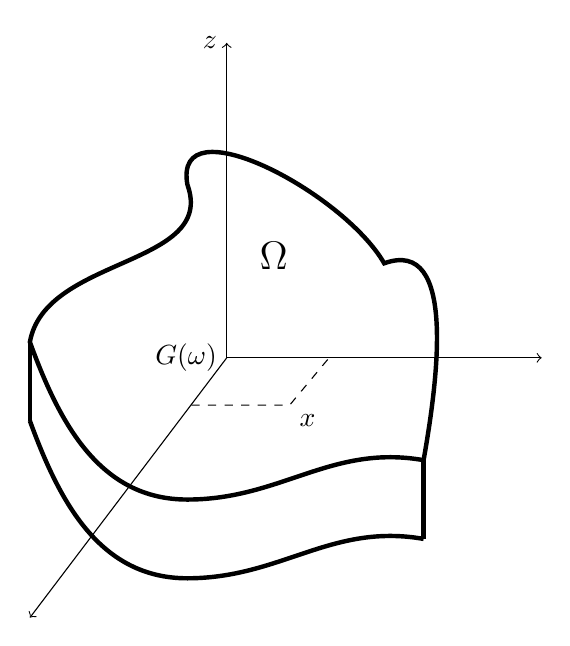
\begin{tikzpicture}
\node[coordinate] (v1) at (-3,3) {};
\node[coordinate] (v2) at (-5,1) {};
\node[coordinate] (v3) at (-3,-1) {};
\node[coordinate] (v4) at (0,-0.5) {};
\node[coordinate] (v5) at (-0.5,2) {};
%\draw  plot[smooth cycle, tension=.7] coordinates {(v5) (v1) (v2) (v3) (v4) (v5)};

\draw [ultra thick] (v1) to [out=290, in=80] (v2) to[out=290, in=180] (v3) to[out=0,in=170] (v4) to[out=80,in=20] (v5) to[out=120,in=100] (v1);

\node[coordinate] (v6) at (-5,0) {};
\node[coordinate] (v7) at (-3,-2) {};
\node[coordinate] (v8) at (0,-1.5) {};

\draw [ultra thick] (v2)--(v6); \draw [ultra thick] (v4)--(v8);
\draw [ultra thick]  (v6) to[out=290, in=180] (v7) to[out=0,in=170] (v8);

\node[coordinate] (v9) at (-2.5,0.8) {};
\node[coordinate] (v10) at (-5.0,-2.5) {};
\node[coordinate] (v11) at (1.5,0.8) {};
\node[coordinate] (v12) at (-2.5,4.8) {};

\draw [->] (v9)--(v10);
\draw [->] (v9)--(v11);
\draw [->] (v9)--(v12);


\node[left] (v9) at (-2.5,0.8) {$G(\omega)$};
\node[left] (v12) at (-2.5,4.8) {$z$};
\node[above left] (v13) at (-1.6,1.8) {\Large $\Omega$};

\node[coordinate] (v14) at (-1.2,0.8) {};
\node[coordinate] (v15) at (-1.7,0.2) {};
\node[coordinate] (v16) at (-2.95,0.2) {};
\draw[dashed] (v16)--(v15)--(v14);

\node[below right] (v15) at (-1.7,0.2) {$x$};

\end{tikzpicture}

%         \includegraphics[width=.8\textwidth]{FloeVue1.tikz} 
%         \caption{Vue d'un floe}
%         \label{fig:floe1}
%     \end{subfigure}
%     % \hfill
%     \begin{subfigure}[b]{0.35\textwidth}
%         \centering
%         % \usetikzlibrary{patterns}

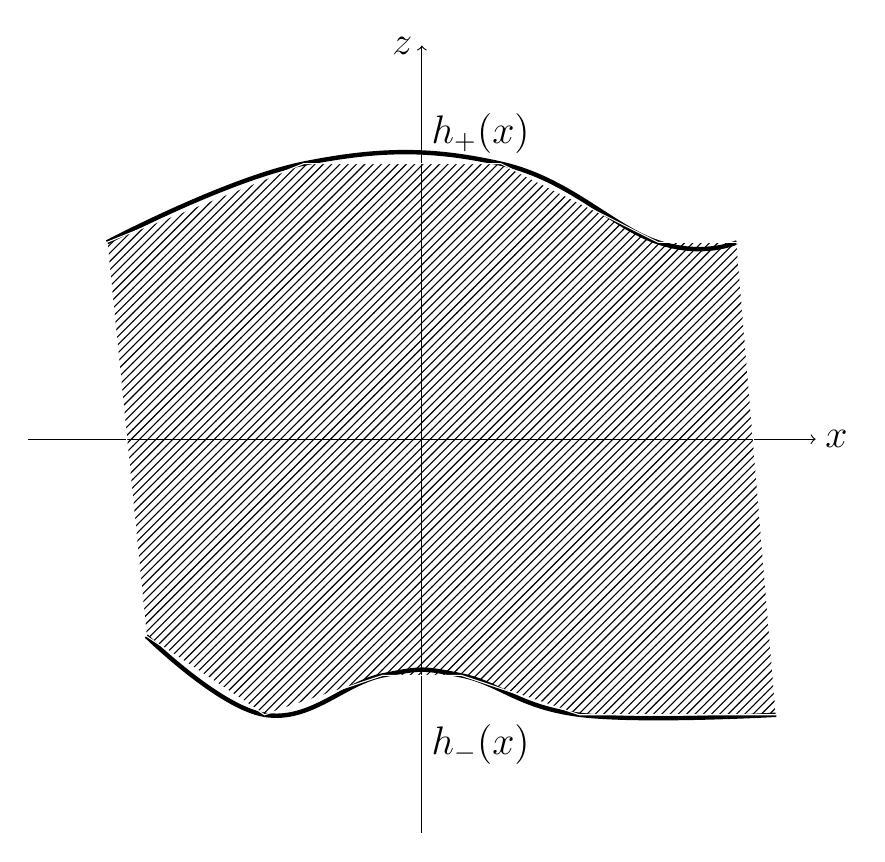
\begin{tikzpicture}

\node[coordinate] (v0) at (0,0) {};
\node[coordinate] (v1) at (-5,0) {};
\node[coordinate] (v2) at (5,0) {};
\node[coordinate] (v3) at (0,-5) {};
\node[coordinate] (v4) at (0,5) {};

\draw [->] (v1)--(v2);
\draw [->] (v3)--(v4);

\node (v5) at (-4,2.5) {};
\node (v6) at (-1.5,3.5) {};
\node (v7) at (1,3.5) {};
\node (v8) at (3,2.5) {};
\node (v9) at (4,2.5) {};
\node (v10) at (-3.5,-2.5) {};
\node (v11) at (-2,-3.5) {};
\node (v12) at (-0.5,-3) {};
\node (v13) at (0.5,-3) {};
\node (v14) at (2,-3.5) {};
\node (v15) at (4.5,-3.5) {};

\draw[ultra thick]  plot[smooth, tension=.7] coordinates {(v5) (v6) (v7) (v8) (v9)};
\draw[ultra thick]  plot[smooth, tension=.7] coordinates {(v10) (v11) (v12) (v13) (v14) (v15)};

\draw [white, pattern=north east lines, xshift=0.5cm,yshift=4.5cm] plot coordinates {(v5) (v6) (v7) (v8) (v9) (v15) (v14) (v13) (v12) (v11) (v10) (v5)};

\node [above right] at (0,3.5) {\Large \bfseries $h_{+}(x)$};
\node [below right] at (0,-3.5) {\Large \bfseries $h_{-}(x)$};
\node [right] at (5,0) {\Large \bfseries $x$};
\node [left] at (0,5) {\Large \bfseries $z$};

\end{tikzpicture} 
%         \includegraphics[width=.8\textwidth]{FloeVue2.tikz} 
%         % \includegraphics[width=2cm]{Figures/FloeVue2.tex}
%         \caption{Coupe transversale}
%         \label{fig:floe2}
%     \end{subfigure}
%        \caption{Illustration de la géométrie d'un floe de glace $\Omega$.}
%        \label{fig:floe}
% \end{figure}

% \noindent On confond le floe au volume qu'il occupe dans l'espace $\Omega$ :
% \[
%     \Omega = \{(x,z) \,|\, x \in \omega \in \Rdeux, \, z \in \,]\hmoins(x), \hplus(x)[ \, \} \,.
% \] 
% Les fonctions $\hmoins$ et $\hplus$ permettent de définir trois quantités (voir \cref{fig:h}) :
% \begin{itemize}
%     \item L'épaisseur moyenne du floe : $\bar{h} =  \sup_{x\in\omega}{\hplus(x)} - \inf_{x\in\omega}{\hmoins(x)}$ ;
%     \item La plus forte épaisseur : $\bar{h}^* = \sup_{x\in\omega}{ \vert \hplus(x) - \hmoins(x) \vert}$ ;
%     \item La plus faible épaisseur : $\underline{h}^* = \inf_{x\in\omega}{ \vert \hplus(x) - \hmoins(x) \vert}$. 
% \end{itemize}

% \begin{figure}[!ht]
%     \centering
%     % \input{Figures/Epaisseur.tikz}
%     \includegraphics[width=.6\textwidth]{h.tikz}
%     \caption{Différentes épaisseurs décrivant un floe de glace. Pour l'instant, afin d'obtenir un floe relativement plat (i.e $\bar{h}$ faible), $\hmoins$ sera pris identiquement nul, et $\hplus$ constant.}
%     \label{fig:h}
% \end{figure}

% \noindent Les vecteurs $\eun$ et $\edeux$ sont liés à $\omega$, et pointent vers un point fixe du bord $\partial \omega$ du floe c-à-d :
% \[
%     \exists \sigma_i \in \partial \omega \, | \, e_i(\omega) = \frac{\sigma_i - G(\omega)}{\Vert \sigma_i - G(\omega) \Vert}, \text{ pour } i \in \{1,2\} \,,
% \]
% où $\Vert \cdot \Vert$ désigne la norme euclidienne de $\Rdeux$. Notons que $\sigma_1 \neq \sigma_2$, et $\eun \cdot \edeux = 0$ de façon à ce que la base orthonormée $(\eun, \edeux)$ soit directe.

% Un floe $\Omega = (\omega, \eun, \edeux, G(\omega), \hmoins, \hplus)$ se déplace sur la mer\footnote{Pour l'instant, la mer est considérée comme un ouvert dans $\Rdeux$. Plus tard, nous prendrons en compte sont épaisseur lorsque nous la modéliserons par une sphère de $\Rtrois$.} $\mathcal{M} \in \Rdeux$. Au temps $t$ après une translation de vecteur $u(t)$ (et de matrice $\mathsf{T}_{u(t)}$), et une rotation de vecteur $\theta(t)$ (et de matrice $\bmat{R}_{\theta(t)}$), on obtient le floe $\Omega (t)$ défini par :
% \[
%     \Omega (t) = (\omega^\prime, \bvec e^1(\omega^\prime), \bvec e^2(\omega^\prime), G(\omega^\prime), \hmoins, \hplus) \,,
% \]
% avec
% $$ 
% \begin{cases}
%     \omega^\prime = \bmat{T}_{u(t)} \bmat{R}_{\theta(t)} \omega \,, \\
%     \bvec e_1(\omega^\prime) = \bmat{T}_{u(t)} \bmat{R}_{\theta(t)} \bvec e_1(\omega) \,, \\
%     \bvec e_2(\omega^\prime) = \bmat{T}_{u(t)} \bmat{R}_{\theta(t)} \bvec e_2(\omega) \,, \\
%     G(\omega^\prime) = \bmat{T}_{u(t)} \bmat{R}_{\theta(t)} G(\omega) \,.
% \end{cases}
% $$
% C'est cette dernière notation mettant en exergue la dépendance avec le temps que nous utiliserons tout au long de ce rapport.

% % \begin{figure}[!h]
% %     \centering
% %     % \input{Figures/Epaisseur.tikz}
% %     \includegraphics[width=.4\textwidth]{FloeMer.tikz}
% %     \caption{Illustration du mouvement d'un floe de glace $F$ dans la mer, après une translation de vecteur $u(t)$ et une rotation d'angle $\theta(t)$, pour obtenir le floe $F_t$. On observe la transformation des propriétés du floe, en partucilier les vecteurs $e_1(\omega)$ et $e_2(\omega)$ qui restent liés au floe.}
% % \end{figure}


% Lors de leur mouvements sur la surface de la mer, les floes se fracturent sous l'effet des vents et des courants océaniques, des phénomènes thermodynamiques, etc. Nous nous intéresserons donc au phénomène de percussion en vue de l'initialisation des fractures dans les floes de glace. Afin de décrire le mouvement des floes de glace sur la mer, nous devons nous munir d'un repère absolu, que nous notons $\mathcal{R}_{abs} = (O, \bvec i, \bvec j, \bvec k)$. Le repère associé au floe $\Omega_i$ sera noté $\mathcal{R}_{\Omega_i} = (O, \bm \eun, \bvec \edeux, \bvec k)$. Dans ce repère absolu, le floe possède 3 degrés de libertés : l'abscisse et l'ordonné de son centre de gravité $G_i(\omega)$, et son orientation donnée par l'angle $\theta_i (t)$ (voir \cref{fig:FloeRepere}). 

% \begin{figure}[!ht]
%     \centering
%     % \input{Figures/Epaisseur.tikz}
%     \includegraphics[width=.5\textwidth]{FloeRepere.tikz}
%     \caption{Positionnement d'un floe de glace $\Omega_i$ dans le repère absolu $\mathcal{R}_{abs}$.}
%     \label{fig:FloeRepere}
% \end{figure}


% %----------------------------------------------------------------------------------------

% \section{Résumé de thèse de M. Rabatel}

% Une fois le modèle défini, il nous faut établir les équations décrivant la dynamique du floe, et celle de son environnement. Les travaux de \citeauthor{rabatel2015thesis} (et plus tard ceux de \citeauthor{balasoiu2020thesis}) ont extensivement traité le problème de modélisation dynamique et de simulation d'un assemblage de floe de glace. Nous résumons ici les principales idées de son raisonnement, tout en présentant l'état de l'art dans ce domaine.

% \subsection{Modélisation théorique de la dynamique des glaces de mer}

% \subsubsection{La cinétique du floe}

% L'approche discrète décrite dans \parencite{rabatel2015thesis} utilise les mêmes notations que celles présentées à la \cref{sec:position}. Les obstacles\footnote{Nous faisons allusion aux obstacles au déplacement des floes. Il peut s'agir des iles, des stations offshore, etc.} sont des floes aux mêmes propriétés que les floes de glace, à la seule différence qu'ils ont une masse (volumique) infinie. Dans \parencite{rabatel2015thesis}, l'auteur travaille dans un repère orthonormé direct $\mathcal{R}_{abs} = (O, \bvec i, \bvec j, \bvec k)$ ; cependant, vu que la mer est considérée plane, le mouvement du floe peut être décrit dans le plan $\mathcal{P} = (O, \bvec i, \bvec j)$. Ensuite, \citeauthor{rabatel2015thesis} désigne la vitesse angulaire du floe $\Omega_i$ par 
% $$
% \bvec{\uptheta}_i(t) = \theta_i(t)\bvec{k} = (0,0,\theta_i(t))^T \,.
% $$
% Soit $P$ (de coordonné $x$) un point quelconque de $\P \subset \Rdeux$. Sa vitesse dans le repère $\R_{abs}$ est donnée est donnée par la formule de Varignon :
% $$
% \dot{P}(t) = \dot{G}_i(t) + \bm{\uptheta}_i(t) \wedge \bvec{G_iP} \,,
% $$
% où le symbole $\wedge$ représente le produit vectoriel dans $\Rtrois$. La masse (constante) du floe rigide indéformable est donnée par 
% $$
% M_i = \rho_i \int_{\Omega_i(t)} h_{i, +} (x) \diff x \,.
% $$
% Ensuite, l'auteur défini :
% \begin{itemize}
%     \item la somme des forces par unité de volume qui s'applique au centre de masse du floe $\Omega_i$ : $$\bvec{F}_i = \rho_i \int_{\Omega_i(t)} \bvec{F}(x) \diff x \,,$$
%     \item le moment cinétique\footnote{Il s'agit d'un moment dû à l'accélération du floe ; alors que le moment dynamique est dû aux forces extérieures. Notons que ces deux vecteurs sont portés par $\bvec{k}$, et peuvent donc être remplacé par des scalaires correspondants.} en $G$ : $$L_i = \rho_i \intO{i} \bvec{GP} \wedge \dot{\bvec{P}}(t) \diff x \,,$$
%     \item le moment dynamique en $G$ : $$\mathfrak{M}_i = \intO{i} \bvec{GP} \wedge \bvec{F}(x) \diff x \,.$$
% \end{itemize}
% Sous le formalisme de Newton-Euler, \citeauthor{rabatel2015thesis} montre que chaque floe $\Omega_i$ vérifie :
% $$
% % \begin{align}
%     \begin{cases}
%         M_i \frac{\diff \dot{\bvec{G}}_i(t)}{\diff t} &= \bvec{F}_i \\
%         \mathcal{I}_i \frac{\diff \dot{\theta}_i(t)}{\diff t} &= \mathfrak{M}_i
%     \end{cases} \,,
% % \end{align}
% $$
% où $\mathcal{I}_i$ représente le moment d'inertie du floe $i$. Ce système se réécrit facilement sous la forme 
% \begin{align}    
%     \mathcal{M}_i \frac{\diff W_i(t)}{\diff t} = \mathcal{H}_i(t) \,,
% \end{align}
% avec 
% $$
% \mathcal{M}_i = 
% \begin{pmatrix}
%     M_i & 0 & 0 \\ 0 & M_i & 0 \\ 0 & 0 & \mathcal{I}_i
% \end{pmatrix} \,, \quad
% W_i(t) = 
% \begin{pmatrix}
%     \dot{\bvec{G}}(t) \\ \dot{\theta}_i(t)
% \end{pmatrix} \,,
% \text{ et } \quad \mathcal{H}_i(t) = 
% \begin{pmatrix}
%     \bvec{F}_i(t) \\ \mathfrak{M}_i(t)
% \end{pmatrix} \,.
% $$
% Pour un système $S$ composé de $n$ floes, le problème précédent doit être satisfait pour tous les floes. \parencite[p.18]{rabatel2015thesis} montre que cela revient à résoudre l'équation
% \begin{align} \label{eq:bilan1}
%     \mathcal{M} \frac{\diff W(t)}{\diff t} = \mathcal{H}(t) \,,
% \end{align}
% avec 
% $$
% \mathcal{M} = (\mathcal{M}_i)_{1\leq i \leq n } \,, \quad
% \mathcal{W}(t) = (\mathcal{W}_i(t))_{1\leq i \leq n } \,, \text{ et } \quad
% \mathcal{M}(t) = (\mathcal{M}_i(t))_{1\leq i \leq n }  \,.
% $$
% L'énergie cinétique du floe $\Omega_i$ quant à elle sera donné par :
% $$
% E_i(t) = \frac{1}{2}M_i \dot{G}_i(t)^2 + \frac{1}{2}\mathfrak{I}_i \dot{\theta}_i(t)^2 \,. 
% $$ 


% \subsubsection{L'interaction entre les floes}


% Le domaine de la mécanique du contact s'est grandement développé ces derniers siècles, avec plusieurs scientifiques qui ont tenté de décrire le phénomène de contact entre des corps rigides. Notons que le problème d'interaction entre les floes est un problème de \textbf{dynamique non-régulière} (contrairement au problème de déplacement des floes entre deux collisions qui lui, est un problème de \textbf{dynamique régulière}). Dans \parencite{rabatel2015thesis}, l'auteur considère deux lois de contact afin de décrire les phénomènes qui se produisent de façon précise :
% \begin{itemize}
%     \item Une \textbf{condition unilatérale de Signorini} : afin de décrire la condition de non-interpénétration ; cette condition est portée par la composante normale\footnote{La composante normale permet aussi d'assurer la dissipation de l'énergie à travers \textbf{la loi de Poisson}.} de la force de contact\footnote{La force de contact est la somme d'une friction tangentielle, et d'une réaction normale.} lors de la collision.
%     \item Une \textbf{loi de friction de Coulomb} : afin de modéliser le comportement de friction pendant une collision. Cette condition est portée par la composante tangentielle de la force de contact.
% \end{itemize}

% \noindent Afin de traiter ces problèmes de contact, deux approches principales ont été d'enveloppées par les scientifiques : l'approche non-régulière et l'approche de régularisation des lois de contact. 

% Parmi les pionniers dans l'\textbf{approche de régularisation} pour la résolution de la condition unilatérale de Signorini, nous pouvons citer Hertz ; Nevins et Whitney \parencite{nevins1972force,whitney1977force}, Moore \parencite{moore1988collision}. Ces méthodes se sont largement répandues dans les études liées à la robotique, à la réalité virtuelle ou encore dans les opérations assistées par ordinateur, pour simuler un grand nombre d’objets en contact en petites ou grandes déformations, comme des habits, des cheveux ou encore des organes (voir \parencite{witkin1990fast,volino1995versatile,baraffandrew,raghupathi2004intestinal}). Concernant la seconde, la loi de friction de Coulomb, la discontinuité entre les phases de glissement et non-glissement a été traitée de différentes façons ; en utilisant la notion de coefficient de restitution, ou des modèles masse-ressorts. 
 
% L'\textbf{approche non-régulière} a été développée en utilisant les concepts d'inclusion différentielles ; ceci afin de traiter la condition de Signorini. Moreau \parencite{moreau1985standard}, Aubin \parencite{aubin2012differential} et Monteiro Marques \parencite{monteiro1985chocs}, ont montré des résultats d’existence et d’unicité de solutions du problème sans friction. Puis, des résultats similaires ont été établis pour le contact unique avec friction (voir \parencite{moreau1986dynamique,monteiro1988inclusoes,panagiotopoulos2012inequality,jean1985system,monteiro1994existence}). Cependant, cette notion d'inclusion différentielle est difficile à manipuler ; c'est, d'après \citeauthor{rabatel2015thesis} la raison pour laquelle le problème du contact multiple avec friction reste encore très peu traité. Il a donc fallu attendre les années 80 avec l'essor des méthodes LCP pour donner un nouveau souffle à l'approche non régulière. Nous pouvons citer ici les travaux de Lötstedt qui fournit des preuves d’existence et d’unicité pour le contact avec la friction de Coulomb (voir \parencite{lotstedt1981coulomb,lotstedt1982mechanical,lotstedt1982time}). On cite aussi Klarbring et Pang, pour leur apport sur le plan des méthodes de programmations. \parencite{rabatel2015thesis} a opté pour cette approche car elle facilite la construction des solutions à partir d’algorithmes tels que ceux de Lemke (voir \parencite{lemke1978some}). \citeauthor{rabatel2015thesis} s'inspire aussi des travaux de Baraff \parencite{baraff1993issues}, qui écrit les forces de contact dans les repères locaux aux points de contact. Ces repères sont définis par la normale et la tangente aux points de contact. La condition de complémentarité se résume comme ceci : "\textit{S’il y a contact alors la réaction est strictement positive et l’accélération relative nulle, et s’il n’y a pas contact l’accélération relative est strictement positive et la réaction nulle.}". Cependant, les travaux de Baraff sur l'existence de solutions sont limités par l'approche accélération-force, et le coefficient de friction qui sont utilisés. En utilisant des formulations en vitesse et impulsion, les chercheurs ont réussi à démontrer l’existence de solutions pour toute configuration à contacts multiples avec n’importe quel coefficient de friction.


% Pour traiter le problème de collision entre les floes, les glaciologues retiennent une multitude de modèles principalement intégrés aux milieux continus. Par exemple, dans les articles de Solomon \parencite{solomon1970study}, ceux de Hibler \parencite{hibler1979dynamic} et ceux de Bratchie \parencite{bratchie1984rheology}, la force résultante des interactions est due à une contrainte interne. On note aussi les modèles basés sur théorie des flux de particules. Dans \parencite{shen1986applying,hopkins1985collisional} par exemple, les collisions ne sont pas détectées précisément et les paramètres décrivant la collision sont déterminés par une méthode de Monte Carlo. L'introduction de ces déformations dans les modèles discrets de la banquise a été initié dans les années 90 par Hopkins \parencite{hopkins1996mesoscale}, et récement par Herman et Wilchinsky \parencite{herman2011molecular,wilchinsky2010effect}. Cependant, elles sont basées sur la régularisation des lois de contact. Avant les travaux de \citeauthor{rabatel2015thesis}, il n'existait pas de modèle discret de banquise en utilisant une dynamique du contact non régulière.


% Le modèle décrit par \parencite[p.5892]{rabatel2015dynamics} utilise deux conditions de complémentarité pour déterminer les vitesses des floes après le contact. La première est une condition de Signorini \parencite{signorini1933sopra} pour s'assurer de la non-interpénétration\footnote{Deux floes s'interpénètre si la "distance" entre ces deux floes est négative.} des floes. Pour décrire ces conditions, il faut au préalable écrire le problème de contact entre floes comme un problème implicite, où les inconnus sont les impulsions après le choc\footnote{Contrairement aux lois de contacts explicites (Hertz, Hooke, Coulomb), les lois implicites ne nécessitent pas la connaissance de la nature du contact entre les floes (glissement ou accroche).}. Pour cette deuxième condition de complémentarité, \citeauthor{rabatel2015thesis} se base sur les travaux de Stewart et Trinkle \parencite{stewart1996implicit} afin d'en extraire une condition qui vérifie la loi de friction de Coulomb. Le problème résultant a ensuite été résolu en utilisant des algorithmes de Lemke. 

% \begin{figure}[!ht]
%     \centering
%     % \input{Figures/Epaisseur.tikz}
%     \includegraphics[width=.28\textwidth]{Collision1.png}
%     \caption{Interaction entre deux floes $\Omega_k$ et $\Omega_l$ au point $P_j$ \parencite[p.26]{rabatel2015thesis}.}
%     \label{fig:Collision1}
% \end{figure}

% Soit $P_j$, ($j \in \{1,\ldots,n\}$) un point de contact entre les floes $\Omega_k$ et $\Omega_l$ (voir \cref{fig:Collision1}). Nous notons $\bvec{F}_{kj}(t)$ la force de contact du floe $\Omega_k$ au floe $\Omega_l$ appliquée en $P_j$. Par convention, une matrice de contact $\bmat{M_c}$ est définie telle que son coefficient $c_kj$ vaut :
% \begin{itemize}
%     \item $0\,\,\,\,\,\, $ si le point de contact $P_j$ n’est pas un point de contact du floe $\Omega_k$ ;
%     \item $-1$ si le point de contact $P_j$ est un point de contact entre les floes $\Omega_k$ et $\Omega_l$ avec $k < l$ ;
%     \item $1\,\,\,\,\,\, $ si le point de contact $P_j$ est un point de contact entre les floes $\Omega_k$ et $\Omega_l$ avec $k > l$.
% \end{itemize}
% En notant $E_k$ l’ensemble des points de contact du floe $\Omega_k$ au temps $t$, \parencite[p.26]{rabatel2015thesis} définit la résultante des forces de contact $\bvec{F}^c_k(t)$, au floe $\Omega_k$ comme :
% $$
% \bvec{F}^c_k(t) = \sum_{j \in E_k} c_{jk} \bvec{F}_{kj}(t) \,.
% $$
% En rajoutent ces forces aux forces extérieures lors du bilan des forces à l'\cref{eq:bilan1}, pour un floe $\Omega_k(t)$, on obtient :
% \begin{align} \label{eq:bilan4}
%     \mathcal{M} \frac{\diff W(t)}{\diff t} = \mathcal{H}(t) + \sum_{j \in E_k} \begin{pmatrix}
%         \bvec{F}_{kj}(t) \\ \bvec{G^kP_j} \wedge \bvec{F}_{kj}(t) 
%     \end{pmatrix} \,.
% \end{align}


% \subsubsection{Formulation en problème linéaire de complémentarité}


% Il existe deux principales manières de formuler le problème du contact entre deux solides rigides. L'auteur de \parencite{rabatel2015thesis} opte pour le formalisme vitesse-impulsion, au détriment du formalisme accélération-force. En effet, l’approche en \textbf{vitesse-impulsion} apporte l’avantage de pouvoir exprimer la force de friction de Coulomb directement par rapport à la vitesse. Il n’est pas nécessaire de connaître la nature du contact. Il nous faut donc définir les notions d'impulsion. Sur un intervalle de temps $\delta t^*$, s’il y a un contact entre les floes $\Omega_k$ et $\Omega_l$ au point $P_j$, nous dirons que le floe $\Omega_k$ a subi un choc provenant du floe $\Omega_l$ au point de contact $P_j$ caractérisé par l’impulsion :
% $$
% \bvec{\mathcal{I}}_{kj} = \int_{\delta t^*} c_{kj} \bvec{F}_{kj}(t) \diff t \,.
% $$ 
% \citeauthor{rabatel2015thesis} fait donc apparaître les impulsions dans les équations des moments \cref{eq:bilan1} pour le floe $\Omega_k$ sur l’intervalle temporel $\delta t^*$ :
% $$
% \mathcal{M}_k \int_{\dtstar} \dot{W}_k(t) \diff t = \int_{\dtstar} \mathcal{H}(t) \diff t + \sum_{j \in E_k} \begin{pmatrix}
%     \bvec{\mathcal{I}}_{kj} \\ \bvec{G_kP_j} \wedge \bvec{\mathcal{I}}_{kj} 
% \end{pmatrix} \,.
% $$
% En écrivant $\dtstar = [t^{-}, t^{+}]$, on peut donc introduire les inconnues $\beta$, $\lambda \in (\Rdeux)^m$ pour le problème de contact  
% \begin{align}
%     \mathcal{M} \left( W(t^{+}) - W(t^{-}) \right) = \int_{\dtstar} \mathcal{H}(t) \diff t + \bmat{B}\beta + \bmat{J}\lambda \,,
% \end{align}
% où $\bmat{B}$ et $\bmat{J}$ sont deux matrices de $(\Rtrois)^{n \times m}$telle que
% \begin{align*}
%     \bmat{B} = (d_{kj})_{\substack{1 \leq k \leq n \\ 1 \leq j \leq m}} \,, \quad d_{kj} = \,
%     \begin{cases}
%         0 \in \Rtrois &\text{ si } P_j \text{ n'est pas un point de contact de } \Omega_k \\
%         \begin{pmatrix}
%             c_{kj} \bvec{T}_{j} \\ c_{kj} \bvec{P}_j\bvec{G}_k \wedge \bvec{T}_j 
%         \end{pmatrix} &\text{ si } P_j \text{ est un point de contact de } \Omega_k
%     \end{cases} \,, \\
%     \bmat{J} = (s_{kj})_{\substack{1 \leq k \leq n \\ 1 \leq j \leq m}} \,, \quad s_{kj} = \,
%     \begin{cases}
%         0 \in \Rtrois &\text{ si } P_j \text{ n'est pas un point de contact de } \Omega_k \\
%         \begin{pmatrix}
%             c_{kj} \bvec{N}_{j} \\ c_{kj} \bvec{P}_j\bvec{G}_k \wedge \bvec{N}_j 
%         \end{pmatrix} &\text{ si } P_j \text{ est un point de contact de } \Omega_k
%     \end{cases} \,.
% \end{align*}
% Les matrices $\bmat{B}$ et $\bmat{J}$ sont obtenues par décomposition des forces de contact dans le repère de contact $\mathcal{R}_{\Omega_j} = (P_j, \bvec{T}_j, \bvec{N}_j)$ (voir \cref{fig:Collision1}).

% Comme précédemment mentionné, afin de modéliser la friction dans une collision qui respecte la loi de Coulomb, \parencite{rabatel2015thesis} se base sur les travaux de Stewart et Trinkle \parencite{stewart1996implicit} qui définissent une condition de complémentarité reliant la composante tangentielle $\beta_j$ de l'impulsion appliquée au point $P_j$, la composante normale $\lambda_j$, la vitesse relative tangentielle du point $P_j$ et le coefficient de friction $\mu$. On introduit le vecteur $\tilde{\beta}$ contenant les composantes de l'impulsion tangentielle dans chacune des directions possible de glissement $\bvec{T}_j$ et $-\bvec{T}_j$. Il devient alors possible de formuler le problème de contact (sur tout le système $S$) sans interpénétration par le problème linéaire de complémentarité :
% \begin{align} \label{eq:bilan3}
% \begin{cases} \,\,
%     \begin{pmatrix}
%         0 \\ \bvec{w} \\ \gamma \\ \sigma 
%     \end{pmatrix} =  
%     \begin{pmatrix}
%         \mathcal{M} &  -\bmat{J} & -\bmat{D} & 0 \\
%         \bmat{J}^T & 0 & 0 & 0 \\
%         \bmat{D}^T & 0 & 0 & \bmat{H} \\
%         0 & \mu & -\bmat{H}^T & 0
%     \end{pmatrix} 
%     \begin{pmatrix}
%         W(t^+) \\ \lambda \\ \tilde{\beta} \\ \alpha
%     \end{pmatrix} + 
%     \begin{pmatrix}
%         \int_{\delta t^*} \mathcal{H}(t) \diff t - \mathcal{M} W(t^{-}) \\ 0 \\ 0 \\ 0
%     \end{pmatrix} \\ \quad
%     \begin{pmatrix}
%         \bvec{w} \\ \gamma \\ \sigma
%     \end{pmatrix} \geq 0 \,, \quad
%     \begin{pmatrix}
%         \lambda \\ \tilde{\beta} \\ \alpha
%     \end{pmatrix} \geq 0 \,, \quad
%     \begin{pmatrix}
%         \bvec{w} \\ \gamma \\ \sigma
%     \end{pmatrix} \cdot
%     \begin{pmatrix}
%         \lambda \\ \tilde{\beta} \\ \alpha
%     \end{pmatrix}  
%      = 0 \,,
% \end{cases}
% \end{align}
% avec
% \begin{align*}
%     &\bvec{w} = \bmat{J}^T W(t^+) \,, \quad
%     \bmat{H}^T = (e_{ij})_{\substack{1 \leq i \leq m \\ 1 \leq j \leq 2m}} \,, \quad \tilde{\beta} = (\tilde{\beta}_j)_{1\leq j \leq m} \,, \quad \lambda = (\lambda_j)_{1 \leq j \leq m} \,, \\
%     &\mu \text{ est la matrice diagonale de diagonale} (\mu_1,\dots, \mu_m) \,,\\
%     &e_{ij} = \begin{cases}
%         1 \text{   si } j = 2(i-1) + 1 \text{ ou } j=2(i-1) + 2 \\
%         0 \text{   sinon} 
%     \end{cases} \,,\\
%     &D = (\bvec{B}_1 \vert - \bvec{B}_1 \vert \ldots \vert \bvec{B}_m \vert -\bvec{B}_m) \, \text{   avec } \bvec{B}_j \text{ la colonne } j \text{ de la matrice } \bmat{B} \,.
% \end{align*}
% Le problème consiste alors à trouver les vitesses après contact $W(t^{+})$, à l’aide des composantes inconnues tangentielle et normale des impulsions dans les repères de contact $(\tilde{\beta}\, \gamma)$, elles-mêmes inconnues du système.


% \subsubsection{Consistance énergétique}


% D'après l'auteur de \parencite[p.42]{rabatel2015thesis}, traiter le problème de contact à partir de lois non régulières ne permet pas d’obtenir des solutions satisfaisant à la fois la non-interpénétration, la friction de Coulomb et une consistance énergétique. En se focalisant sur la consistance énergétique, \citeauthor{rabatel2015thesis} a subdivisé le problème en deux : une phase de compression et une phase de décompression suivant la loi de Poisson. La \textbf{phase de compression} modélise la capacité maximale des floes à emmagasiner, par la déformation, une partie ou la totalité de l’énergie cinétique transmise lors du contact. L'impulsion normale $\lambda^c$ calculée durant cette phase (en résolvant le problème de complémentarité (\cref{eq:bilan3})) correspond a un coefficient de restitution $\varepsilon = 0$. Les impulsions obtenues durant cette phase correspondent à celles nécessaire pour éviter la non-interpénétration, et correspondent donc a une énergie cinétique maximale emmagasinée. La \textbf{phase de décompression} correspond à la restitution partielle ou complète de l’énergie cinétique emmagasinée par la déformation des floes. L’impulsion lors de cette phase, notée $\lambda^d$, est déterminée par $\lambda^d = \varepsilon \lambda^c$ (l’hypothèse de Poisson \parencite{glocker1995multiple}). Durant la phase de décompression, \citeauthor{rabatel2015thesis} a donc opté pour la consistance énergétique et la non-interpénétration avec la solution :
% $$
% W^N = (1 + \varepsilon)W^{c} - \varepsilon W(t^{-}) \,,
% $$
% où $W^c$ représente les vitesses des floes après la phase de compression, et $\varepsilon$ le coefficient de restitution pour les contacts considérés inélastiques.

% % \subsubsection{Traitement des conditions aux bords}

% \subsubsection{Le modèle de l'environnement}


% L’environnement est l’ensemble des forces extérieures qui agissent sur les floes hormis les forces de contact qui sont décrites dans la partie précédente. Ces principales forces sont:
% \begin{itemize}
%     \item La force de Coriolis $\bvec{\mathfrak{F}}_c$ donnée pour un floe $\Omega_i(t)$ par:
%     $$
%     \bvec{\mathfrak{F}}_{c,i}(t) = -f\bvec{k} \wedge \dot{\bvec G}_i(t) \,,
%     $$
%     avec $f$ le paramètre de Coriolis et $\bvec{k}$ le vecteur dirigé vers le haut du repère absolu $\mathcal{R}_{abs}$.
%     \item Les forces de trainée associées au vent $\bvec{\tau}_a(t)$ et celle associée à l'océan $\bvec{\tau}_w(t)$: 
%     \begin{align*}
%         \bvec{\tau}_a(t) &= \rho_a C_a \Vert \bvec{U}_a(t) \Vert \bvec{U}_a(t) \,, \\        
%         \bvec{\tau}_w(t,P) &= \rho_w C_w \Vert \bvec{U}_w(t) - \dot{P}(t) \Vert \left(\bvec{U}_w(t) - \dot{P}(t) \right) \,,
%     \end{align*}
%     avec $\rho$ la masse volumique du fluide (l'indice $a$ pour l'air et $w$ pour l'eau) et $C$ un coefficient de traînée sans dimension (voir [HI86]) ; $\bvec{U}_a$, $\bvec{U}_w$, $\dot{P}(t)$ respectivement la vitesse du vent à l'interface glace/fluide, la vitesse du courant oceanique à l'interface glace/fluide, et la vitesse d'un point $P$ du floe. 
% \end{itemize}

% Le modèle de dynamique régulière définit en \cref{eq:bilan1} peut se voire expliciter:
% \begin{align*}
%     \begin{cases}
%             M_i \frac{\diff \dot{\bvec{G}}_i(t)}{\diff{t}} &= M_i \mathfrak{F}_{c,i}(t) + \int_{\Omega_i(t)} \bvec{\tau}_a(t) + \bvec{\tau}_w(t,P) \diff s \,,\\
%             \mathcal{I}_i \frac{\diff \dot{\theta}_i(t)}{\diff t} &= \int_{\Omega_i(t)} \bvec{G}_i\bvec{P} \wedge \left(\bvec{\tau}_a(t) + \bvec{\tau}_w(t,P)\right) \diff s \,.
%     \end{cases}
% \end{align*} 
% L'algorithme décrivant en détail le processus de collision ainsi que la consistance énergétique se trouve à la page 43 du document \parencite{rabatel2015thesis}.


% \subsection{Méthodes numériques et algorithmiques pour la résolution du problème}
 
% \subsubsection{Discrétisation temporelle}

% Pour simuler la dynamique des floes de glace soumis a des forces extérieures et possiblement des collisions, il faut intégrer la dynamique régulière (entre deux collisions), et la dynamique non régulière ; et il existe deux principales méthodes pour la discrétisation en temps dans de tels problèmes. La méthode \textit{\textbf{time-stepping}} (voir \parencite{acary2013projected} pour les schéma de Moreau \parencite{moreau1986dynamique,jean1999non}, et de Schatzman-Paoli \parencite{paoli2002numerical,paoli2002numerical2} par exemple, pour lesquels une convergence a pu être exhibée à partir de la convergence en graphe de Moreau \parencite{moreau1978approximation}) ; comparé aux autres méthodes, la méthode \textit{time-stepping} traite mieux les points d'accumulation \parencite[p.58]{rabatel2015thesis} ; et est plus performante sur des problèmes de multiples contacts. Cependant, \citeauthor{rabatel2015thesis} pour le schéma \textit{\textbf{event-driven}} pour sa précision dans la localisation des collisions et sa facilité de manipulation. En plus, elles permettent d’utiliser des schémas d’intégration existant d’ordre élevé pour des équations différentielles ordinaires. Le seuil de collision choisi est suffisamment grand pour éviter de traiter les collisions une par une. Le schéma utilisé pour intégrer l'équation \cref{eq:bilan1} est un schéma du type Euler explicite, pour sa facilité d’implémentation, sa facilité à prédire la localisation en espace et en temps des futures collisions et enfin, sa capacité à dépasser les problèmes de points d’accumulation. 

% La simulation par la méthode \textit{event-driven} demande la définition d'un pas de temps maximal pour lequel le schéma reste stable. Le pas de temps $\Delta t_max$ sera utilisé si aucune collision n'est détectée entre les instants $t$ et l'instant $t + \Delta t_max$. En se référant au un modèle idéalisé 1D (voir \parencite[p.49]{rabatel2015thesis}), \citeauthor{rabatel2015thesis} distingue deux critères pour la stabilité du schéma numérique au temps $t$ :
% \begin{itemize}
%     \item lorsque la vitesse caractéristique des floes $V_c(t) = N_a \bvec{U}_a(t) + \bvec{U}_w(t)$ est constante sur l'intervalle de simulation $I$, alors pour :  
%     \begin{align} \label{eq:dtmax1}
%         \Delta t \leq \Delta t_{max} = \min{ \left(\frac{\rho}{2 \vert \bvec{U}_a(t) \vert \sqrt{\rho_a C_a \rho_w C_w}} \,, \,\frac{2K_t}{L_t} \right)}
%     \end{align}
%     avec 
%     $$
%     \text{avec } L_t = \rho^{-1} \rho_w C_w \left( N_a^2 \bvec{U}_a^2 + (N_a\bvec{U}_a + 2 \bvec{U}_w)^2 \right) \,, \text{et } K_t = \vert V_c(t) \vert \text{ constant, }
%     $$
%     le schéma est stable c-à-d. $\dot{\bvec{G}} (t + \Delta t) \in [-K_t, K_t] = [-K_{t + \Delta t}, K_{t + \Delta t}]$ ;
%     \item lorsque les variations de $V_c(t)$ entraînent une augmentation de $K_t$ au cours du temps. La propriété de stabilité reste vérifiée car $$\dot{\bvec{G}} (t + \Delta t) \in [-K_t, K_t] \in [-K_{t + \Delta t}, K_{t + \Delta t}] \,;$$
%     \item lorsque les variations de $V_c(t)$ entraînent une diminution stricte de $K_t$ au cours du temps, alors la condition de stabilité dans les deux cas précédents ne peut être vérifiée. \citeauthor{rabatel2015thesis} introduit donc une seconde définition de la stabilité pour traiter ce cas. Il remarque que pour 
%     \begin{align} \label{eq:dtmax2}
%     \Delta t_{max} \leq \begin{cases}
%         \frac{-2x}{\tilde{L}_t^{-}} \text{  si  } x \in  ]-\infty, K_{t+\Delta t}] \\
%         \frac{-2x}{-\tilde{L}_t^{+}} \text{  si  } x \in  ]K_{t+\Delta t}, +\infty]
%     \end{cases}\end{align}
%     avec \begin{align*} \tilde{L}_t^{-} =  \rho^{-1} \rho_w C_w \left[ N_a^2 \bvec{U}_a(t+\Delta t)^2 - (\bvec{U}_w(t + \Delta t) - x)^2 \right] \\ \tilde{L}_t^{+} =  \rho^{-1} \rho_w C_w \left[ N_a^2 \bvec{U}_a(t+\Delta t)^2 + (\bvec{U}_w(t + \Delta t) - x)^2 \right] \,,
%      \end{align*}
%     on a la diminution de la vitesse des floes.
% \end{itemize} 
% En conclusion, pour une vitesse infinitésimale initiale $\dot{G}(0) \in [-K_0, K_0]$, pour tout $t \in I$, et pour tout $\Delta t_{max}$ vérifiant les \cref{eq:dtmax1,eq:dtmax2}, nous avons les vitesses des floes majorées par :
% $$
% \max_{t \in I}{K_t}
% $$
% \citeauthor{rabatel2015thesis} choisi donc de prendre 
% $$
% \Delta t_{max} = \min{ \left( \frac{3}{4} \frac{ -2 \left( \max_{t \in I}{K_t} \right)}{ \max_{t \in I}{\tilde{L}_t^{-}}}, \frac{3}{4} \frac{2 \left( \max_{t \in I}{K_t} \right) }{ \max_{t \in I}{-\tilde{L}_t^{+}}}, \frac{\rho}{2 \left(  \max_{t \in I}{  \vert \bvec{U}_a(t) \vert } \right)  \sqrt{\rho_a C_a \rho_w C_w}} \right)}
% $$
% pour s'assurer que le modèle idéalisé vérifie les critères de stabilité définis. 
% Notons que le procédé global d’intégration de la dynamique pour le modèle se situe à la figure 2.2 du document \parencite[p.60]{rabatel2015thesis}, le schéma est repris à la \cref{fig:Algo1}.

% \begin{figure}[!ht]
%     \centering
%     \includegraphics[width=.62\textwidth]{Algo1.png}
%     \caption{Procédé global d’intégration de la dynamique pour notre modèle \parencite[p.60]{rabatel2015thesis}.}
%     \label{fig:Algo1}
% \end{figure}


% \subsubsection{Détection des collisions en espace}

% Des deux méthodes principales utilisées dans la littérature pour la détection des voisins, \citeauthor{rabatel2015thesis} a choisi la méthode de \textbf{hiérarchie de volumes englobants} pour sa facilité de mise en place et pour son efficacité même avec de grands ratios de tailles. L'alternative était la méthode de \textbf{partitionnement de l'espace} qui elle, souffre de plusieurs défauts non surmontables pour le modèle développé. Les méthodes de volumes englobants consistent à englober le contour de l’objet par des volumes à des échelles de plus en plus fines pour améliorer la détection.

% \subsubsection{Détection des contacts en temps}

% Il s'agit ici de trouver le pas de temps optimal c’est-à-dire un pas de temps $\Delta t$ pour lequel la configuration des floes ne contenant pas d’interpénétrations sur l’intervalle de temps $[t, t + \Delta t]$ et, pour tout $\varepsilon > 0$, contient au moins une interpénétration sur l’intervalle de temps $[t + \Delta t, t + \Delta t + \varepsilon]$ \parencite[p.87]{rabatel2015thesis}.
% Lorsque le critère de collision n’est pas vérifié, \citeauthor{rabatel2015thesis} montre qu'il suffit de prendre 
% $$
% \Delta t_{i,j} = -\frac{-\delta_{i,j(t)} - tol_3}{\bvec{A}_{ij}(t) \cdot \left( \dot{G}_i(t) - \dot{G}_j(t) \right)} \,,
% $$
% avec 
% $$
% \bvec{A}_{i,j}(t) = \frac{C_{0,i}(t) - C_{0,i}(t)}{d\left(C_{0,i}(t), C_{0,i}(t) \right)} \,, \text{ et  } \quad tol_3 = \frac{\xi}{20} \,.
% $$
% Lorsque le critère de collision est vérifié, il faut plutôt prendre 
% $$
% \Delta t_{i,j} = \frac{\min{\left( \eta_i, \eta_j \right) - tol_3}}{\Gamma(t)} \,,
% $$
% avec 
% $$
% \Gamma(t) = \max{\left( \Vert \dot{Q}_i^{i,j}(t) \Vert \,, \, \Vert \dot{Q}_j^{j,i}(t) \Vert  \right)} \,,
% $$
% où $\dot{Q}_i^{i,j}$ représente la distance parcourue par un point de $\Omega_i (t)$ relativement à $\Omega_j (t)$.

% Une fois ce $\Delta t_{i,j}$ assurant la non-interpénétration trouvé, on peut donc choisir 
% $$
% \Delta t = \min{\left( \Delta t_{max} \,, \min_{ \substack{ (i,j) \in \left\{ 1,\ldots,n \right\}^2 \\ i \neq j}}{\Delta t_{i,j}} \right)} \,.
% $$
% Le lecteur est renvoyé au document \parencite[p.91]{rabatel2015thesis} pour plus de détails sur la détection des contacts en temps.

% \subsubsection{Construction des repères de contacts}

% La construction d'un repère de contact n'est effectuée que lorsque le contact entre deux floes $\Omega_k$ et $\Omega_l$ est \textbf{linéique} \parencite[p.79]{rabatel2015thesis}, ou \textbf{ponctuel} et le vecteur porté par les points en contacts appartient au cône normal de $P$. La normale $\bvec{N}$ est alors déterminée comme le vecteur unité dirigé par $\bvec{PQ}$. Si $Q$ n’est pas unique, on se retrouve dans la situation où il peut exister plusieurs repères de contact pour un point de contact. Dans les autres cas, le repère de contact associé au point $P$ n’est pas construit et $P$ n’est pas considéré dans le traitement des contacts \parencite[p.80]{rabatel2015thesis}. L'algorithme de détection des points de contacts afin de construire les repère de contact est explicité dans le document \parencite[p.76]{rabatel2015thesis}. 


% \subsubsection{Simulation des événements collisions}

% Une fois les voisins détectés et les repères de contact construits, on peut passer à la prochaine étape qui consiste en la simulation des évènements de collisions. Ici, plusieurs choix s'offrent à nous : les méthodes dites de \textbf{régularisations}, les méthodes dites \textbf{itératives}, et les méthodes dites \textbf{de pivots} \parencite[p.82]{rabatel2015thesis}. La première catégorie est adaptée aux modèles régularisants, ce qui n'est le cas de notre modèle. La deuxième par contre a extensivement été utilisée dans la littérature ; on peut citer Moreau \parencite{moreau1988unilateral,moreau1999numerical,jean1999non}, Aitken \parencite{aitken1950iv}. Malheureusement, dès que la matrice $A$ du problème de complémentarité à résoudre n'est plus symétrique, ce deuxième groupe de techniques ne s'avère pas efficace. \citeauthor{rabatel2015thesis} choisi donc l'algorithme de Lemke pour lequel il existe des preuves de convergence lorsque la matrice $A$ est co-positive. Bien qu'il soit performant, il faut néanmoins noter que l’algorithme de Lemke étant une technique globale, c’est-à-dire traitant les contacts simultanément, il ne garantit pas une bonne propagation du contact \parencite[p.82]{rabatel2015thesis}.

% \subsubsection{Optimisations}

% La première optimisation apporté est celle sur les distances de collision : deux floes sont en contact si la distance entre eux n'est pas nulle, mais supérieure à un seul appelée \textbf{distance de collision}.

% La deuxième concerne la condition de non-interpénétration \parencite[p.85]{rabatel2015thesis}. En cas de congestion, il est difficile que les floes décollent après contact. En exigeant que $\bmat{J}^T W(t^+) > 0$ après collision, on risque ne pas avoir de solution pour le problème linéaire de complémentarité associé. \citeauthor{rabatel2015thesis} relaxe donc la condition de Signorini en définissant un réel $c$, et l'ensemble des vitesses admissibles devient donc :
% $$
% V_c = \left\{ w \in \mathbb{R}^{3n} \, | \, \bmat{J}^T w \geq c \right\} \,.
% $$
% Une troisième optimisation concernant la définition de la \textbf{notion d'erreur} et de \textbf{tolérance} a été implémentée. La quatrième consiste en la résolution d'un LCP en trois tentatives (avec trois algorithmes de Lemke différents) même si cela augmente les coups de calculs \parencite[p.86]{rabatel2015thesis}. Si cette optimisation ne s'avère pas suffisance, une dernière optimisation consiste en la modification aléatoire de certains coefficients de la matrice $A$, la permutation des lignes afin d'éviter des zéros sur la diagonale, ou encore l'utilisation de la notion de \textbf{contact actif}.


% \subsection{Validations et exploitations du modèle}

% Les résultats ont été validés à travers plusieurs expériences. Nous citons des exemples classique tels que la \textbf{boîte glissante}, le \textbf{berceau de Newton}, le \textbf{canon de Newton}, la \textbf{balle rebondissante}, etc. Le modèle a ensuite été validé sur des scénarios simples de dérive libre soumise à des courants océanique et atmosphérique et des scénarios simples de collision. En effet, il a été vérifié que le comportement d’un objet simulé est cohérent avec le comportement théorique et avec les observations. Les principes physiques suivants ont ainsi pu être testé par \citeauthor{rabatel2015thesis} :
% \begin{itemize}
%     \item la conservation de la symétrie d’une configuration ;
%     \item la satisfaction du modèle de Coulomb ;
%     \item le traitement d’un point d’accumulation ;
%     \item la cohérence temporelle ou la propagation des ondes de choc ;
%     \item la conservation de l’énergie cinétique.
% \end{itemize} 
% Des telles exploitations telles que la dérive dans un canal étroit, pour des floes en bassins a été étudié (voir \cref{fig:Derive,fig:DeriveSol}). Aussi, la dérive soumise à un vent et un courant variable avec des vitesses du vent provenant de \textbf{ERAinterim}, à partir du modèle glace de mer et océan \textbf{TOPAZ} a été étudiée.

% \begin{figure}[!ht]
%     \centering
%     \includegraphics[width=.28\textwidth]{Derive.png}
%     \caption{Configuration à l’instant initial pour le scénario de dérive dans un canal étroit \parencite[p.124]{rabatel2015thesis}.}
%     \label{fig:Derive}
% \end{figure}

% \begin{figure}[!ht]
%     \centering
%     \includegraphics[width=.68\textwidth]{DeriveSol.png}
%     \caption{Quelques résultats obtenus à deux heures différentes de la configuration des floes pour différentes valeurs du coefficient de restitution $\varepsilon$ \parencite[p.126]{rabatel2015thesis}.}
%     \label{fig:DeriveSol}
% \end{figure}

% \subsection{Discussion}
% Bien que les travaux de \citeauthor{rabatel2015thesis} ont été testés et validés sur plusieurs configurations différentes, il reste néanmoins des points qui ne sont pas traités, et qui ont très clairement été soulignés dans la thèse \parencite{rabatel2015thesis} :
% \begin{enumerate}
%     \item Le modèle ne gère pas la rhéologie\footnote{La rhéologie est l'étude de la déformation et de l'écoulement de la matière sous l'effet d'une contrainte appliquée.} de la glace : les floes sont des solides purement rigides (ils ne se déforment pas) et la dissipation d’énergie cinétique durant la collision est décrite en utilisant un coefficient purement empirique collision.  
%     \item La loi de contact utilisée pour le glissement (voir \parencite{stewart1996implicit}), bien que très riche, ne prends pas en compte toutes les vitesses possibles de déplacement. La construction d’une loi qui donnerait accès à la région entière, demanderait de prendre en compte un grand nombre de phénomènes intrinsèques aux contacts. Leur compréhension et leur rôle à chacun est difficile à déterminer. 
%     \item Les coefficients de friction et de restitution utilisées sont limitants. En réalité, il n’est pas possible de prendre en compte ou d'interpréter mathématiquement certains effets lors du contact ; par exemple, avec la dispersion de l'énergie (voir \parencite{nguyen2014multiple}). Cette dispersion est la conséquence de certains effets vibratoires à travers une chaîne de contact. Seuls les effets de dissipation dus aux phénomènes locaux comme l’endommagement, la viscosité ou la plasticité sont pris en compte à travers l’utilisation des coefficients de restitution et de friction.
%     \item Les vitesses obtenues après la phase de décompression afin d'assurer la dissipation de l'énergie cinétique possèdent une faiblesse : elles ne sont solutions que sous certaines conditions, comme le fait que les chocs soient frontaux et qu’il n’y ait pas d’apport des forces extérieures autres que les forces de contact durant la collision \parencite[p.41]{rabatel2015thesis}.
% \end{enumerate}

% %----------------------------------------------------------------------------------------



%----------------------------------------------------------------------------------------

\section{Résumé de thèse de D. Balasoiu}

Les travaux de D. Balasoiu concernent la modélisation et la simulation du comportement mécanique de floes de glace \parencite{balasoiu2020thesis}. Il s'agit d'une amélioration des travaux de M. Rabatel, S. Labbé, et J. Weiss \parencite{rabatel2015thesis,rabatel2015dynamics} prenant en compte la fracture des floes. Précisément, ce travail se focalise sur l’initiation de la fracture, ainsi que la prédiction du chemin que la fracture emprunte. Jusqu’à présent, les floes étaient considérés comme des corps rigides ; dans sa thèse, \citeauthor{balasoiu2020thesis} les considère comme des corps élastiques. Son travail est divisé en deux parties. Il commence par proposer un modèle efficace pour la fracture fragile d’un floe de glace, lorsque celui-ci est soumis à un déplacement de son bord (i.e. à une condition au bord de type Dirichlet). Puis, dans un second temps, il cherche à obtenir l’expression du déplacement au bord d’un floe qui percute un autre floe ou une structure solide.

\subsection{Théorie de la fracture : état de l’art} 
 
La théorie de fracture la plus répendue de nos jous est due à A.A. Griffith  Dans ses travaux[Gri21], in invalide les résultats que C. Inglis [Ing13] qui ne tennaient pas en compte la taille de la fracture ; il présente donc la croissance d'une faille comme une compétition d'énergie entre l'énergie élastique\footnote{Énergie relâchée lorsqu’un défaut subit un accroissement} et l'énergie de surface\footnote{Énergie nécessaire à la création des deux nouvelles surfaces – les bords de la fissure}. 

\subsection{Discussion}

Plusieurs hypothèses sont faites dans la thèse :
\begin{enumerate}
    \item Le modèle suppose que les floes sont d’épaisseur négligeable devant leur extension horizontale ; autrement dit, les déformations du floe de glace peuvent être étudiées en deux dimensions.
    \item Le modèle restreint l’ensemble des fractures admissibles à celui des segments de droites.
\end{enumerate}       %% État de l'art
% % Chapter 4

\chapter{Travaux et apports} % 4th chapter title

\label{Chapter4} % For referencing the chapter elsewhere, use \ref{Chapter4} 


%----------------------------------------------------------------------------------------


\section{Les missions du poste}

\begin{itemize}
    \item L'état de l'art de la partie précédente fait partie des missions.
    \item Modélisation
    \item Simulation
\end{itemize}

Nous souhaitons étudier le comportement mécanique d'un floe après collision avec un autre floe. Les étapes de travail envisagées sont les suivantes:
\begin{enumerate}
    \item Ecire les systèmes differentiels pour les deux floes juste après le choc: pour l' instant on peut considérer que l'un des floes est immobile (celà revient au même si l'on exprimes les vitesses dans un repère lié à ce floe).
    \item On exprime l'EDO vérifiée par les solutions, c'est à dire $q$ pour le premier floes, et $p$ pour le second.
    \item On pourra ensuite simuler ces EDP limites et trouver les valeurs de $p$ et $q$. Autrement dit, on connait la position de chaque point du réseau au temps final.
    \item Si on connait $p$ et/ou $q$, on connait la condition de Dirichlet sur le floe concerné, et on peut ainsi exprimer le déplacement et la possible fracture du floe. 
\end{enumerate}







\section{Présentation des résultats obtenus}










\subsection{Modélisation et simulation 1D}









\subsubsection{Modélisation du déplacement d'un floe isolé}

Avant d'entamer la question de la percussion, étudions le comportement d'un floe de glace 1D modélisé par un réseau de ressorts (1 ressort, 1 dispositif viseux, et 2 noeuds) (voir \cref{fig:deplacement1d}).
\begin{figure}[!h]
    \centering
    \frame{\includegraphics[width=0.6\textwidth]{Deplacement1D-Systeme.png}}
    \caption{Floe de glace 1D modélisé par un réseau de ressorts. Le floe est isolé de toutes forces extérieurs. Les varaibles $x_1$ et $x_2$ traduisent les déplacemnts des noeuds de gauche et de droite respectifs. À l'instant initial, les masses sont soumises aux vitesses $v_0$ et $v'_0$ indiquées.}
    \label{fig:deplacement1d}
\end{figure}


\begin{figure}[!h]
    \begin{subfigure}[b]{0.33\textwidth}
        \centering
        \frame{\includegraphics[width=\textwidth]{Deplacement1D-Masse1.png}}
        \caption{Sur la masse $m$ de gauche.}
    \end{subfigure}
%     \hfill
    \begin{subfigure}[b]{0.3\textwidth}
        \centering
        \frame{\includegraphics[width=\textwidth]{Deplacement1D-Masse2.png}}
        \caption{Sur la masse $m$ de droite.}
    \end{subfigure}
       \caption{Bilan des forces appliquée sur les noeuds du système. Les valeurs indiquées sont les intensitées (positives) des forces (par exemple juste après l'instant initial, on a $x_1 > 0$, et $x_2 < 0$ d'où $k(x_1-x_2) > 0$).}
       \label{fig:bilan0}
\end{figure}


\noindent Un bilan des forces effectué sur les deux noeuds du floe (voir \cref{fig:bilan0}) permet d'obtenir les équations suivantes:
\begin{align}
    \begin{dcases}
    m\ddot x_1 = - k(x_1 - x_2) - \mu(\dot x_1 - \dot x_2) \,,\\
        m \ddot x_2 =  k(x_1 - x_2) + \mu(\dot x_1 - \dot x_2) \,. 
    \end{dcases}
\end{align}
En remarquant que $m\neq 0$, on passe à la forme matricielle qui s'écrit:
\begin{align}
    \myvec{\ddot{x}_1}{\ddot{x}_2} = 
      \underbrace{ \frac{k}{m} \mymat{-1}{1}{1}{-1}}_{B} \myvec{x_1}{x_2}
    + \underbrace{\frac{\mu}{m} \mymat{-1}{1}{1}{-1}}_{C} \myvec{\dot{x}_1}{\dot{x}_2} \,.
\end{align}
On pose ensuite la matrice par blocs:
\[ E = \mymat{0}{I_2}{B}{C}  =  \begin{pmatrix}
    0 & 0 & 1 & 0 \\ 0 & 0& 0& 1 \\ -\frac{k}{m} & \frac{k}{m} & -\frac{\mu}{m} & \frac{\mu}{m} \\ \frac{k}{m} & -\frac{k}{m} & \frac{\mu}{m} & -\frac{\mu}{m}
\end{pmatrix}   \in \mathbb{R}^{4\times 4} \,, \quad \text{où} \quad I_2 = \mymat{1}{0}{0}{1} \in \mathbb{R}^{2\times 2} \,. \]
On pose maintenant $Y = (x_1, x_2, \dot{x}_1, \dot{x}_2) \in \mathbb{R}^4$, et on reprend la condition initiale pour obtenir le système de Cauchy:
\begin{align} \label{eq:dep1d}
    \begin{dcases}
        \dot{Y}(t)= E Y(t) \,, \\
        Y_0 = Y(t_0) = (0,0,v_0,-v'_0)^T \,.
    \end{dcases}
\end{align}

La solution numérique est présentée dans à la \cref{fig:simudept1d} (voir fichier \verb|code/simu1D/Deplacement1D-1.ipynb| pour plus de détails). La plus grosse remarque à faire du point de vue numérique est que lorsque $v_0 \neq v'_0$, les vitesses convergent vers $0$, mais les déplacements diverge.
\begin{figure*}[!h]
    \centering

    \begin{subfigure}[t]{0.45\textwidth}
        \centering
        \includegraphics[width=\textwidth]{SimuDeplacement1D1.png}
        \caption{$v_0=v'_0 = 0.8$}
    \end{subfigure}
    \begin{subfigure}[t]{0.45\textwidth}
        \centering
        \includegraphics[width=\textwidth]{SimuDeplacement1D2.png}
        \caption{$v_0= 0.6$ et $v'_0 = 0.8$}
    \end{subfigure}

    \caption{Simulation du déplacement 1D d'un floe avec $m=1$, $k=18$, $\mu=1.3$, $t_{f}=5$. En règle générale, on observe le ralentissement du système et une convergence des déplacements vers l'état d'équilibre $Y_{eq}= (0,0,0,0)$ lorsque $v_0 = v'_0$.}
    \label{fig:simudept1d}
\end{figure*}

Avec $t_0= 0$, la solution analytique de ce système d'EDO du premier ordre à coefficients constants est unique et est donnée par.
\begin{align}
    Y(t) = \exp(tE)Y_0 \,.
\end{align}
Nous obtenons le théorème suivant:
\begin{theorem}[Convergence du modèle 1D isolé] \label{th:div1D}
    Les déplacements $x_1$ et $x_2$ des noeuds du floe 1D convergent si et seulement si leurs vitesses initiales sont des vecteurs opposés.
\end{theorem}

\begin{proof}

Le calcul des solution analytique est plus délicat. Il faudrait calculer l'exponentielle de la matrice $E$. Pour celà, nous devons diagonaliser (ou du moins trogonaliser) la matrice $E$. Son polynome caractéristique est donné par:
\begin{align*}    
\text{det}(E-\lambda I_4) &&&= \begin{vmatrix}
    -\lambda & 0 & 1 & 0 \\ 0 & -\lambda & 0& 1 \\ -\frac{k}{m} & \frac{k}{m} & -\frac{\mu}{m}-\lambda & \frac{\mu}{m} \\ \frac{k}{m} & -\frac{k}{m} & \frac{\mu}{m} & -\frac{\mu}{m} -\lambda
\end{vmatrix}, \\
    &&&= \frac{\lambda^2}{m} \left( m\lambda^2 + 2\mu\lambda + 2k \right).
\end{align*}
Posons $\Delta = 4\mu^2 - 8km$. On distingue deux cas:
\begin{itemize}
    \item Si $\Delta \geq 0$: on pose $\lambda_1 = \frac{-\mu - \sqrt{\mu^2 - 2km}}{m}$ et $\lambda_2 = \frac{-\mu + \sqrt{\mu^2 - 2km}}{m}$;
    \item Si $\Delta < 0$: on pose $\lambda_1 = \frac{-\mu - i\sqrt{2km - \mu^2}}{m}$ et $\lambda_2 = \frac{-\mu + i\sqrt{2km - \mu^2}}{m}$.
\end{itemize}
Nous avons donc exhiber les trois valeurs propres de notre matrice: $\lambda_0 = 0$, $\lambda_1$, et $\lambda_2$. Avec $\lambda$ désignant l'une des valeurs propres, on recherche les vecteurs $x = (x_1, x_2, x_3, x_4)^T \in \mathbb{R}^4$ appartenant aux sous espaces propres $E_\lambda$. On a:
\begin{align} \label{eq:espacepropre}
    Ex = \lambda x \Rightarrow \begin{dcases}
        x_3 = \lambda x_1 \\
        x_4 = \lambda x_2 \\
        -(k + \mu \lambda + m \lambda^2) x_1 + (k + \mu \lambda) x_2 = 0 \\
        (k + \mu \lambda) x_1 - (k + \mu \lambda + m \lambda^2) x_2 = 0
    \end{dcases}
\end{align}
\begin{itemize}
    \item Pour $\lambda = 0$, l'\cref{eq:espacepropre} revient à:
    \begin{align*}
        \begin{dcases}            
        x_3 = 0 \\
        x_4 = 0 \\
        x_1 - x_2 = 0
        \end{dcases}
    \end{align*} 
    On en déduit $E_0 = \text{vect}\{ e_1 \}$, avec $e_1 = (1,1,0,0)^T$.
    \item Pour $\lambda = \lambda_1, \lambda_2$, on remarque que $k + \mu \lambda + m \lambda^2 = - (k + \mu \lambda)$. l'\cref{eq:espacepropre} revient donc à:
    \begin{align*}
        \begin{dcases}            
        x_3 = \lambda x_1 \\
        x_4 = \lambda x_2 \\
        x_1 + x_2 = 0
        \end{dcases}
    \end{align*} 
    On en déduit donc $E_{\lambda_1} = \text{vect}\{ e_3 \}$, avec $e_3 = (1,-1,\lambda_1,-\lambda_1)^T$; et $E_{\lambda_2} = \text{vect}\{ e_4 \}$ avec $e_4 = (1,-1,\lambda_2,-\lambda_2)^T$.
\end{itemize}
La meutilisicté arithmetique de $\lambda = 0$ est differente de sa multiplicité géometrique. La matrice $E$ n'est donc pas diagonalisable. Son polynome caractéristique étant scindé, nous alons la trigonaliser. On pose donc une base $\mathcal{B}' = (v_1, v_2, v_3, v_4)$ dans laquelle la matrice $E$ s'exprime par:
\begin{align*}
    P^{-1}EP = \begin{pmatrix}
        0 & a & b & c \\ 0 & 0 & d & e \\ 0 & 0 & \lambda_1 & f \\ 0 & 0 & 0 & \lambda_2
    \end{pmatrix},
\end{align*}
où $P$ est la matrice de passage de la base canonique de $\mathbb{R}^4$ (notée $\mathcal{B}$) à $\mathcal{B}'$. On a:
\begin{itemize}
    \item Dans $\mathcal{B}'$, le vecteur $v_1$ s'écrit $v_1 = (1,0,0,0)^T$ et on a $P^{-1}EP v_1 = 0$. $v_1$ est donc le vecteur propre associé à $0$ et on prend $v_1 = e_1 = (1,1,0,0)^T$ dans $\mathcal{B}$;
    \item Dans $\mathcal{B}'$, le vecteur $v_2$ s'écrit $v_2 = (0,1,0,0)^T$ et on a $P^{-1}EP v_2 = a v_1$. On retourne dans $\mathcal{B}$ en posant $v_2 = (x_1, x_2, x_3, x_4)^T$ pour obtenir le système:
    \begin{align*}
        E v_2 = a v_1 \Rightarrow
        \begin{dcases}            
        x_3 = a  \\
        x_4 = a  \\
        x_1 - x_2 = 0
        \end{dcases}.
    \end{align*} 
    Avec $a = 1$, on écrit $v_2 = e_2 = (1,1,1,1)^T$.
    \item Dans $\mathcal{B}'$, le vecteur $v_3$ s'écrit $v_1 = (0,0,1,0)^T$ et on a $P^{-1}EP v_1 = \lambda_1 v_1 + bv_1 + d v_2$. En posant $b=d=0$, $v_1$ devient un vecteur propre associé à $\lambda_1$ et on prend $v_3 = e_3 = (1,-1,\lambda_1,-\lambda_1)^T$ dans $\mathcal{B}$;
    \item De facon similaire, on obtient $v_4 = e_4 = (1,-1,\lambda_2,-\lambda_2)^T$ en posant $c=e=f=0$.
\end{itemize}
Nous avons donc trigonaliser la matrice $E$, et on écrit :
\begin{align*}
    P^{-1}EP = A, \text{avec} A = \begin{pmatrix}
        0 & 1 & 0 & 0 \\ 0 & 0 & 0 & 0 \\ 0 & 0 & \lambda_1 & 0 \\ 0 & 0 & 0 & \lambda_2
    \end{pmatrix}, \text{  } P = \begin{pmatrix}
        1 & 1 & 1 & 1 \\ 1 & 1 & -1 & -1 \\ 0 & 1 & \lambda_1 & \lambda_2 \\ 0 & 1 & -\lambda_1 & -\lambda_2
    \end{pmatrix}, \text{ et } P^{-1} = \frac{1}{2}\begin{pmatrix}
        1 & 1 & -1 & -1 \\ 0 & 0 & 1 & 1 \\ \frac{\lambda_2}{\lambda_2-\lambda_1} & -\frac{\lambda_2}{\lambda_2-\lambda_1} & -\frac{1}{\lambda_2-\lambda_1} & \frac{1}{\lambda_2-\lambda_1} \\ -\frac{\lambda_1}{\lambda_2-\lambda_1} & \frac{\lambda_1}{\lambda_2-\lambda_1} & \frac{1}{\lambda_2-\lambda_1} & -\frac{1}{\lambda_2-\lambda_1}
    \end{pmatrix}.
\end{align*}
La matrice $A$ se décompose en somme d'une matrice diagonale et d'une matrice nilpotente $A = D+N$ avec:
\begin{align*}
    D = \begin{pmatrix}
        0 & 0 & 0 & 0 \\ 0 & 0 & 0 & 0 \\ 0 & 0 & \lambda_1 & 0 \\ 0 & 0 & 0 & \lambda_2
    \end{pmatrix}, \text{ et } N = \begin{pmatrix}
        0 & 1 & 0 & 0 \\ 0 & 0 & 0 & 0 \\ 0 & 0 & 0 & 0 \\ 0 & 0 & 0 & 0
    \end{pmatrix}.
\end{align*}
En posant $E = P(D+N)P^{-1}$, nous pouvons facilemtn calculer $\forall t \in \mathbb{R}$, $\exp(tE) = P\exp(tD)\exp(tN)P^{-1}$. Ce calcul délicat donne (à l'aide du logiciel de calcul symbolique $\verb|Symbolab|$):
\begin{align*}
    \exp(tE) = \tiny \frac{1}{2(\lambda_2 - \lambda_1)}\begin{pmatrix} 
        \lambda_2e^{t\lambda_1} + \lambda_2 - \lambda_1 - \lambda_1e^{t\lambda_2} & -\lambda_2e^{t\lambda_1} + \lambda_2 - \lambda_1 + \lambda_1e^{t\lambda_2} & t(\lambda_2 -\lambda_1) - e^{t\lambda_1} + e^{t\lambda_2} & t(\lambda_2 -\lambda_1) + e^{t\lambda_1} - e^{t\lambda_2} \\
         -\lambda_2e^{t\lambda_1} + \lambda_2 - \lambda_1 + \lambda_1e^{t\lambda_2} & \lambda_2e^{t\lambda_1} + \lambda_2 - \lambda_1 - \lambda_1e^{t\lambda_2} & t(\lambda_2 -\lambda_1) + e^{t\lambda_1} - e^{t\lambda_2} & t(\lambda_2 -\lambda_1) - e^{t\lambda_1} + e^{t\lambda_2} \\
          \lambda_1\lambda_2 (e^{t\lambda_1} - e^{t\lambda_2}) & \lambda_1\lambda_2 (e^{t\lambda_2} - e^{t\lambda_1})  & -\lambda_1e^{t\lambda_1} + \lambda_2 - \lambda_1 + \lambda_2e^{t\lambda_2} & \lambda_1e^{t\lambda_1} + \lambda_2 - \lambda_1 - \lambda_2e^{t\lambda_2} \\
          \lambda_1\lambda_2 (e^{t\lambda_2} - e^{t\lambda_1})  & \lambda_1\lambda_2 (e^{t\lambda_1} - e^{t\lambda_2})  & \lambda_1e^{t\lambda_1} + \lambda_2 - \lambda_1 - \lambda_2e^{t\lambda_2} & -\lambda_1e^{t\lambda_1} + \lambda_2 - \lambda_1 + \lambda_2e^{t\lambda_2}
    \end{pmatrix}.
\end{align*}
Rappelons nous que la solution du problème de Cauchy \cref{eq:dep1d} est donnée par $Y(t) = \exp(tE)Y_0$, avec $Y_0 = (0,0,v_0,-v'_0)$. Le calcul du déplacement $x_1$ donne:
\begin{align} \label{eq:solreel}
    x_1(t) = \frac{t}{2}\left( v_0 - v'_0 \right) \textcolor{red}{+} \frac{e^{t\lambda_1} - e^{t\lambda_2}}{2(\lambda_2 - \lambda_1)}\left( v_0 + v'_0 \right).
\end{align}
Le cas où $\Delta < 0$ (à étudier dans $\mathbb{C}$) peut se ramener au cas réel (dans $\mathbb{R}$) en posant $\lambda_1 = \alpha + i \beta$ et $\lambda_2 = \alpha - i \beta = \bar{\lambda}_1$ (avec $\alpha = -\frac{\mu}{m}$ et $\beta = -\frac{\sqrt{2km - \mu^2}}{m}$). En remarquant que $\sin(\beta t) = \frac{e^{i\beta t} - e^{-i\beta t}}{2i}$, on obtient:
\begin{align} \label{eq:solcomplexe}
    x_1(t) = \frac{t}{2}\left( v_0 - v'_0 \right) \textcolor{red}{+} \frac{e^{\alpha t} \sin(\beta t)}{2\beta} \left( v_0 + v'_0 \right).
\end{align}
Les \cref{eq:solreel,eq:solcomplexe} permettent d'observer que le déplacement $x_1$ ne converge pas lorsque $t \rightarrow +\infty$, à moins que $v_0 = v'_0$, ce qui est observé à la \cref{fig:simudept1d}. On tire les mêmes conclusions pour $x_2$ en effectuant un raisonnement similaire.

\end{proof}








\subsubsection{Collision parfaitement inélastique avec un floe encastré à l'instant initial}

Nous effectuons ici une modélisation 1D de notre problème. Un floe est modélisé par un système masse-ressort de deux nœuds. Le floe 1 est immobilisé face au mur, et le floe 2 approche à la vitesse $\bvec{v}_0$. On identifie les nœuds $q_0$ et $p_0$ de la section précédente à leur masses respectives $m$ et $m'$ (voir \cref{fig:contact1d}).
\begin{figure}[!h]
    \centering
    \frame{\includegraphics[width=0.8\textwidth]{Percussion1D-Systeme}}
    \caption{Contact 1D parfaitement inélastique entre deux floes. Le floe percuté étant immobile et coincé au mur avant le choc.}
    \label{fig:contact1d}
\end{figure}

\noindent On suppose que durant la dynamique non régulière, les masses $m$ et $m'$ en contact forment une seule masse\footnote{Cette simplification a pour principal avantage de supprimer le traitement de la force de contact entre les deux masses.}
$m+m'$ dont
le déplacement est donné par la variable $x_1(t)$. Le déplacement de la masse $m'$ à l'autre bout du floe percuteur est nommé
$x_2(t)$. La masse $m$ qui est fixée au mur ne sera pas étudiée ici. Nous faisons à présent le bilan des forces qui
s'exercent ces
deux masses.
\begin{figure}[!h]
     \begin{subfigure}[b]{0.4\textwidth}
         \centering
         \frame{\includegraphics[width=\textwidth]{Percussion1D-Masse1}}
         \caption{Sur $m+m'$.}
         \label{fig:bilan11}
     \end{subfigure}
%     \hfill
     \begin{subfigure}[b]{0.3\textwidth}
         \centering
         \frame{\includegraphics[width=\textwidth]{Percussion1D-Masse2}}
         \caption{Sur $m'$.}
         \label{fig:bilan12}
     \end{subfigure}
        \caption{Bilan des forces appliquée sur les noeuds du système. Les valeurs indiquées sont les intensitées
            (positives) des forces durant une phase imaginée de compression des ressorts ($\bvec{v}_0 <0$ et donc
            $x_1 <0$). Pour obtenir l'intesité de la force de rappel du ressort $k'$, on peut imaginer $x_1$ imobile
            (on aura $x_2 < 0$, d'où $x_1 - x_2 > 0$) (voir \parencite{homodeling}).}
        \label{fig:bilan}
\end{figure}

\noindent En orientant convenablement le système (voir \cref{fig:contact1d}), on applique la loi de Newton-Euler linéaire
pour obtenir le système suivant et ses conditions initiales \footnote{J'ai des doutes sur cette condition
initiale. La vitesse initiale de $x_1$ est-elle vraiment nulle?}:
\begin{align}
    \begin{dcases}
    (m+m')\ddot x_1 = -kx_1 - \mu \dot x_1 + k'(x_2 - x_1) + \mu'(\dot x_2 - \dot x_1) \\
        m' \ddot x_2 =  -k'(x_2 - x_1) - \mu'(\dot x_2 - \dot x_1) 
    \end{dcases}
\end{align}
À l'instant initial $t_0$, on a le système suivant
\begin{align} \label{eq:percussion1d}
    \begin{dcases}
    (x_1(t_0), x_2(t_0)) = (0,0) \\
    (\dot x_1(t_0), \dot x_2(t_0)) = (0,-v_0)
    \end{dcases}
\end{align}
En posant $X = (x_1, x_2)^T \in \mathbb{R}^2$, l' \cref{eq:percussion1d} devient
\begin{align}
    \underbrace{\mymat{m+m'}{0}{0}{m'}}_{A} \myvec{\ddot{x}_1}{\ddot{x}_2} = \underbrace{\mymat{-\mu -
    \mu^\prime}{\mu'}{\mu'}{-\mu'}}_{B}
    \myvec{\dot{x}_1}{\dot{x}_2} + \underbrace{\mymat{-k-k'}{k'}{k'}{-k'}}_{C} \myvec{x_1}{x_2} \,.
\end{align}
Puisque $m, m'\neq 0$, la matrice $A$ est inversible et on obtient au final le problème de Cauchy suivant:
\begin{align} \label{eq:percussion1d2}
    \begin{dcases}
        \ddot{X}(t) = B' \dot{X}(t) + C'X(t) \,, \\
        (X(t_0), \dot X (t_0)) = \left( \myvec{0}{0}, \myvec{0}{-v_0} \right) \,,
    \end{dcases}
\end{align}
avec $B' = A^{-1}B$ et $C' = A^{-1}C$.

\noindent Il s'agit la d'un système d'EDO du deuxième ordre à coefficients constants. Transformons le en un système du premier ordre pour
une résolution plus aisée. On pose donc $Y= (X, \dot X)^T = (x_1, x_2, \dot{x}_1, \dot{x}_2)^T \in \mathbb{R}^4$ et le
système
\ref{eq:percussion1d2}
devient
\begin{align} \label{eq:systeme1d}
    \begin{dcases}
        \dot{Y}(t)= E Y(t) \\
        Y_0 = Y(t_0) = (0,0,0,-v_0)^T
    \end{dcases}
\end{align}
avec la matrice par blocs \[ E = \mymat{0}{I_2}{C'}{B'} \,, \] où $I_2$ désigne la matrice identité de
$\mathbb{R}^{2\times2}$.

\noindent Avec $t_0= 0$, la solution de ce système d'EDO du premier ordre à coefficients constants est unique et est donnée par
\begin{align}
    Y(t) = \exp(tE)Y_0
\end{align}

La résolution analytique du système passe par le calcul de l'exponentielle de la matrice $E \in \mathbb{R}^4$, ce qui s'avère difficile du à la taille de ladite matrice. Nous optons donc pour une solution numérique (voir figure \cref{fig:simucontact1d} issue du notebook $\verb|code/simu1D/Percussion1D-1.ipynb|$ ) \ldots
\begin{figure}[!h]
    \centering
    \includegraphics[width=0.4\textwidth]{SimuPercussion1D.png}
    \caption{Simulation de la percussion 1D entre deux floes avec $m=1$, $m'=1$, $k=16$, $k'=5$, $\mu=6$,
        $\mu'=2$, $v_0=-1.0$, $t_{f}=32$. On observe effectivement le ralentissement du système et une convergence
        vers l'état d'équilibre $Y_{eq}= (0,0,0,0)$.}
    \label{fig:simucontact1d}
\end{figure}

\noindent Pour certaines valeurs (specifiquement de $\mu$ et $\mu'$), on constate que le système converge vers son état d'équilibre attendu $Y_{eq} = (0,0,0,0)$. Il nous reste dans cette section:
\begin{enumerate}
    \item Calculer analytiquement et numériquement tous les état d'équilibres $Y_{eq} \in \ker(E)$; distinguer les états stables des autres.
    \item Calculer analytiquement l'exponentielle de la matrice $E$, et donner l'expression de la solution; déduire la condition sur les parametres pour que le système converge vers l'état d'équilibre voulu.
\end{enumerate} 







\subsubsection{Collision parfaitement inélastique sans présence du mur}

Contrairement au cas étudié dans la section précédente, le mur est supprimé dans cette section. On obtient donc une troisième variable $x_3$ décrivant le comportement du noeud qui était rattaché au mur. La schéma régissant ce système est donnée à la \cref{fig:contact1d2}. Le bilan des forces appliquées aux noeuds est présenté à la \cref{fig:bilan2}.

\begin{figure}[!h]
    \centering
    \frame{\includegraphics[width=0.8\textwidth]{Percussion1D-Systeme-2}}
    \caption{Contact 1D parfaitement inélastique entre deux floes. Le floe percuté étant non immobile (et non coincé au mur) avant le choc. On représnte également les variables $x_1$, $x_2$, et $x_3$ décrivant les movements de chaque noeud.}
    \label{fig:contact1d2}
\end{figure}

\begin{figure}[!h]
    \begin{subfigure}[b]{0.25\textwidth}
        \centering
        \frame{\includegraphics[width=\textwidth]{Percussion1D2-Masse1.png}}
        \caption{Sur $m$.}
        \label{fig:bilan12}
    \end{subfigure}
%     \hfill
    \begin{subfigure}[b]{0.31\textwidth}
        \centering
        \frame{\includegraphics[width=\textwidth]{Percussion1D2-Masse2}}
        \caption{Sur $m+m'$.}
        \label{fig:bilan22}
    \end{subfigure}
%     \hfill
    \begin{subfigure}[b]{0.23\textwidth}
        \centering
        \frame{\includegraphics[width=\textwidth]{Percussion1D2-Masse3}}
        \caption{Sur $m'$.}
        \label{fig:bilan32}
    \end{subfigure}
       \caption{Bilan des forces appliquée sur les noeuds du système. On procède de facon similaire à \cref{fig:bilan} pour obtenir les sens et les intensités de ces forces.}
       \label{fig:bilan2}
\end{figure}

\noindent Comme précédement, nous appliqons les lois de Newton pour obtenir:
\begin{align}
    \begin{dcases}
    m\ddot x_1 = -k(x_1 - x_2) - \mu (\dot x_1 - \dot x_2) \,, \\
    (m+m')\ddot x_2 = k(x_1 - x_2) + \mu (\dot x_1 - \dot x_2) - k'(x_2 - x_3) - \mu'(\dot x_2 - \dot x_3) \,, \\
        m' \ddot x_3 =  k'(x_2 - x_3) + \mu'(\dot x_2 - \dot x_3) \,. 
    \end{dcases}
\end{align}
Sous forme matricielle, on a
\begin{align}
    \underbrace{\mybigmat{m}{0}{0}{0}{m+m'}{0}{0}{0}{m'}}_{A} \mybigvec{\ddot{x}_1}{\ddot{x}_2}{\ddot{x}_3} =  
    \underbrace{\mybigmat{-k}{k}{0}{k}{-k-k'}{k}{0}{k'}{-k'}}_{B} \mybigvec{x_1}{x_2}{x_3} + 
    \underbrace{\mybigmat{-\mu}{\mu}{0}{\mu}{-\mu-\mu'}{\mu'}{0}{\mu'}{-\mu'}}_{C} \mybigvec{\dot{x}_1}{\dot{x}_2}{\dot{x}_3} \,.
\end{align}
Puisque $m, m'\neq 0$, la matrice $A$ est inversible. En posant $X = (x_1, x_2, x_3)^T \in \mathbb{R}^3$, le système d'EDO revient à l' \cref{eq:percussion1d22} suivante:
\begin{align} \label{eq:percussion1d22}
        \ddot{X}(t) = B' X(t) + C'\dot{X}(t) \,, 
\end{align}
où $B' = A^{-1}B$ et $C' = A^{-1}C$. On pose ensuite $Y= (X, \dot X)^T \in \mathbb{R}^6$ et le système \cref{eq:percussion1d22} devient 
\begin{align} \label{eq:systeme1d2}
        \dot{Y}(t)= E Y(t)
\end{align}
avec $$ E = \mymat{0}{I_3}{B'}{C'} \,.$$


Remarquons qu'en enlevant le mur à gauche du domaine (voir \cref{fig:contact1d}), le système est devenu isolé. Nous pouvons donc appliquer la conservation de la quantité de mouvement pour identifier la vitesse de l'ensemble $m+m'$ après collision et fixation de la masse $m'$ (à vitesse $\bvec{v}_0$) sur la masse $m$ (de vitesse $\bvec{v}'_0$)\footnote{Le vecteur $\bvec{v}'_0$ n'est pas marqué à la \cref{fig:contact1d2} (i.e. $\bvec{v}'_0 = 0$). L'introduction de ce vecteur permet de généraliser le problème.}. Pour simplifier les calculs, nous considérons les floes comme des solides rigides. La vitesse de l'ensemble juste après collision est notée $v_f$, et les quantités de mouvement avant et après choc sont notées $P_{\text{avant}}$ et $P_{\text{après}}$. On a :
\begin{align*}
    & \quad P_{\text{avant}} = P_{\text{après}} \\
    \Rightarrow & \quad 2m \bvec{v}_0 + 2m'\bvec{v'}_0 = (2m + 2m') \bvec{v}_f \\
    \Rightarrow & \quad \bvec{v}_f = \frac{m \bvec{v}_0 + m'\bvec{v'}_0}{m+m'}
\end{align*} 

\noindent On introduit ces conditions initiales dans l'\cref{eq:systeme1d2} pour obtenir le système de Cauchy ci-bas. Le résulat de la simulation est présenté à la figure \cref{fig:simucontact1d2} (issue du notebook $\verb|code/simu1D/Percussion1D-2.ipynb|$). 
\begin{align} \label{eq:systeme1d3}
    \begin{dcases}
        \dot{Y}(t)= E Y(t) \,, \\
        Y(t_0) = Y_0 = -v_f(0,0,0,1,1,1) \,.        
    \end{dcases}
\end{align}

\begin{figure}[!h]
    \centering
    \begin{subfigure}{0.45\textwidth}
        \centering
        \includegraphics[width=\textwidth]{SimuPercussion1D2.png}
        \caption{$k=3$}
    \end{subfigure}
    \begin{subfigure}{0.45\textwidth}
        \centering
        \includegraphics[width=\textwidth]{SimuPercussion1D2NonConv.png}
        \caption{$k=23$}
    \end{subfigure}

    \caption{Simulation de la percussion 1D entre deux floes (sans présence du mur) avec $m=1$, $m'=1$, $k'=22$, $\mu=6$, $\mu'=2$, $v_0=-1.8$, $t_{f}=5$. Sous certaines conditions (forte dissipation, raideur du floe percuté élevée, etc.), on observe le ralentissement du système et une convergence vers l'état d'équilibre $Y_{eq}=(0,0,0,0,0,0)$.} 
    \label{fig:simucontact1d2}
\end{figure}

\noindent La \cref{fig:simucontact1d2} permet d'observer la nuance avec le problème de contact parfaitemetn inélastique. Il est difficile de distinguer les cas qui aboutissent à une convergences des déplacements de ceux qui divergent. Observons donc à présent un problème de contact inélastique avec séparation des masses.




\subsubsection{Collision inélastique avec séparation des masses}

Reprennons le cas du contact 1D et étudions ce qui se passe durant l'intervale de temps $\tdelta = [\tmoins, \tplus]$ de la collision. Cette fois, pour étudier la dynamique non régulière, nous décidons de séparer les masses $m$ et $m'$ en contact (et ce même durant le contact). Le système résultant est très similaire aux deux cas traités précédemment (\cref{fig:contact1d,fig:contact1d2}), et nous le présentons à la \cref{fig:contact1d3} ci-bas, et son bilan de forces à la \cref{fig:bilan3}.

\begin{figure}[!h]
    \centering
    \frame{\includegraphics[width=0.8\textwidth]{Percussion1D-Systeme-3}}
    \caption{Contact 1D inélastique entre deux floes. Durant le choc, les nœuds $m$ et $m'$ en contact sont étudiés séparement. On représnte les variables $x_1$, $x_2$, $x_3$, et $x_4$ décrivant les movements de chaque noeud.}
    \label{fig:contact1d3}
\end{figure}


\begin{figure}[!h]
    \begin{subfigure}[b]{0.30\textwidth}
        \centering
        \frame{\includegraphics[width=\textwidth]{Percussion1D3-Masse1.png}}
        \caption{Sur $m$ de gauche ($x_1$).}
        \label{fig:bilan13}
    \end{subfigure}
%     \hfill
    \begin{subfigure}[b]{0.35\textwidth}
        \centering
        \frame{\includegraphics[width=\textwidth]{Percussion1D3-Masse2}}
        \caption{Sur $m$ de droite ($x_2$).}
        \label{fig:bilan23}
    \end{subfigure}
%     \hfill
    \begin{subfigure}[b]{0.35\textwidth}
        \centering
        \frame{\includegraphics[width=\textwidth]{Percussion1D3-Masse3}}
        \caption{Sur $m'$ de gauche ($x_3$).}
        \label{fig:bilan33}
    \end{subfigure}
%     \hfill
    \begin{subfigure}[b]{0.30\textwidth}
        \centering
        \frame{\includegraphics[width=\textwidth]{Percussion1D3-Masse4}}
        \caption{Sur $m'$ de droite ($x_4$).}
        \label{fig:bilan43}
    \end{subfigure}
       \caption{Bilan des forces appliquée sur les $4$ noeuds du système. On procède de facon similaire aux \cref{fig:bilan,fig:bilan2} pour obtenir les sens et les intensités de ces forces. $F_c$ représente la force de contact dont l'intensité est inconnue.}
       \label{fig:bilan3}
\end{figure}

\noindent Comme précédement, nous appliqons les lois de Newton pour obtenir:
\begin{align}
    \begin{dcases}
    m\ddot x_1 = -k(x_1 - x_2) - \mu (\dot x_1 - \dot x_2) \,, \\
    m\ddot x_2 = k(x_1 - x_2) + \mu (\dot x_1 - \dot x_2) - F_c \,, \\
    m'\ddot x_3 = - k'(x_3 - x_4) - \mu'(\dot x_3 - \dot x_4) + F_c \,, \\
        m' \ddot x_4 =  k'(x_3 - x_4) + \mu'(\dot x_3 - \dot x_4) \,. 
    \end{dcases}
\end{align}
On additionne membre à membre les équations régissant les mouvements de $x_2$ et $x_3$ pour éliminer la force de contact $F_c$ et obtenir le système:
% \begin{align}\label{eq:systeme3test}
    \begin{subnumcases}{}
    m\ddot x_1 = -k(x_1 - x_2) - \mu (\dot x_1 - \dot x_2) \,, \label{eq:sys1D1}\\
    m\ddot x_2 + m'\ddot x_3 = k(x_1 - x_2) + \mu (\dot x_1 - \dot x_2) - k'(x_3 - x_4) - \mu'(\dot x_3 - \dot x_4) \,, \label{eq:sys1D2} \\
        m' \ddot x_4 =  k'(x_3 - x_4) + \mu'(\dot x_3 - \dot x_4) \,. \label{eq:sys1D3}
    \end{subnumcases}
% \end{align}
Remarquons que ce système reviens au même systeme étudié dans la partie précédente en posant $x_2(t) = x_3(t) $ p.p. En effet, durant la phase de contact, les massess $m$ et $m'$ peuvent etrs étudiées comme une unique masse $m+m'$. La grosse diffculté qui ressort de cette modélisation est la définitions de la vitesse initiale de l'ensemble $m+m'$. Celà dit, nous cherchons à trouver les vitessses $\dot x_1(\tplus)$, $\dot x_2(\tplus)$, $\dot x_3(\tplus)$ et $\dot x_4(\tplus)$ immédiatemetn après la collision. De par la ressemblance de ce modèle avec celui de la section précédente (voir \cref{eq:systeme1d2}), nous réutilisons les quantités $\dot x_1$ et $\dot x_4$ données par ce système (l'\cref{eq:systeme1d2} dans lequel $x_2$ et $x_3$ sont confondus). On peut se permertre une telle approximation car $x_1$ et $x_4$ n'interviennent pas directemetn dans la collision. De plus, la quantité $k(x_1 - x_2) + \mu (\dot x_1 - \dot x_2) - k'(x_3 - x_4) - \mu'(\dot x_3 - \dot x_4)$
% \begin{align}
%     I = k(x_1 - x_2) + \mu (\dot x_1 - \dot x_2) - k'(x_3 - x_4) - \mu'(\dot x_3 - \dot x_4)    
% \end{align}
est aussi calculé suivant le modèle \cref{eq:systeme1d2} (voir l'article \parencite{tommasino2020effect} pour une modélisation similaire). Il ne nous reste véritablement que $2$ inconnue dans notre dynamique irrégulière.

\noindent Intégrons l'équation (\ref{eq:sys1D2}) entre les instants $\tmoins$ et $\tplus$. On obtient:
\begin{align}    \label{eq:debuteq1}
    \int_{\tmoins}^{\tplus} m\ddot x_2 + m'\ddot x_3 \diff t = \underbrace{\int_{\tmoins}^{\tplus} k(x_1 - x_2) + \mu (\dot x_1 - \dot x_2) - k'(x_3 - x_4) - \mu'(\dot x_3 - \dot x_4) \diff t}_{I} \,.
\end{align}
Afin d'éviter toute confusion, nous notons $v_0 = \dot{x}_2(\tmoins)$ et $v'_0 = \dot{x}_3(\tmoins)$ les vitesses des noeuds en contact avant collision, et $V_0 = \dot{x}_2(\tplus)$ et $V'_0 = \dot{x}_3(\tplus)$ les vitesses après contact. L'équation \cref{eq:debuteq1} devient donc:
\begin{align} \label{eq:crammer1}
    mV_0 + m'V'_0 = I + mv_0 + m'v'_0 \,.
\end{align}
À présent, nous pouvons étudier l'énergie cinétique du système à travers le coefficient de restitution $\varepsilon$ \footnote{Le coefficient de restitution est le même que celui utilisé dans la thèse \parencite{rabatel2015thesis}.}. On suppose (algébriquement) que les noeuds prennent des directions indiquées à la \cref{fig:contact1dapres}. 
\begin{figure}[!h]
    \centering
    \frame{\includegraphics[width=0.6\textwidth]{Percussion1D3-Apres.png}}
    \caption{Situation après contact 1D.}
    \label{fig:contact1dapres}
\end{figure}

\noindent On obtient l'\cref{eq:crammer2}:
\begin{align} \label{eq:crammer2}
    - V_0 + V'_0 = \varepsilon (v_0 - v'_0) \,.
\end{align}
Le système de Cramer qui découle des \cref{eq:crammer1,eq:crammer2} permet d'obtenir les expressions:
\begin{align}
    V_0 = \frac{I + (m+\varepsilon m')v_0 + (1-\varepsilon)m'v'_0}{m+m'} \,, \quad V'_0 = \frac{I + (1-\varepsilon)mv_0 + (m'+\varepsilon m)v'_0}{m+m'}\,.
\end{align}

Nous faisons donc ici la grosse hypothèse que \underline{le mouvement de $x_2$ et $x_3$ devient uniforme après la collision}. Une fois leur vitesses "initiales"\footnote{Ces vitesses sont les vitesses de départ pour le deuxième phase de la percussion.} obtenues, on calcule donc les déplacements des différents noeuds des réseaux, et les fractures éventuelles qui s'en suivent. 

\paragraph{Analyse du modèle.} Observons le premier floe de plus près:
\begin{itemize}
    \item Son noeud de gauche $x_1$ a pour vitesse $v_0$ avant et le choc et conserve cette vitesse après le choc;
    \item Son noeud de droite $x_2$ a pour vitesse $v_0$ avant le choc, mais passe de facon discontinue à $V_0$ apres le choc.
\end{itemize}
N'ayant aucune garantie que les vecteurs vitesses $v_0$ et $V_0$ seront opposés immédiatemetn après le choc, nous ne pouvons garantir la convergence de ce modèle (voir \cref{th:div1D}). Ce modèle dégénère (probablement) après la première collision. Effectuons à présent une modélisation 2D et observons si le même problème se repète.

%%-------Pas vrai
% Pour $\varepsilon \neq 0$, l'\cref{eq:crammer2} permet de constater que $V_0 = V'_0$ si et seulement si $v_0 = v'_0$. En se basant sur le \cref{th:div1D}, nous pouvons donc énoncer le corrolaire suivant:

% \begin{corollary} \label{cr:div1D}
%     Le modèle de collision inélastique 1D avec séparation des masses converge si les vitesses des noeuds avant le choc sont des vecteurs opposés.

%     Le modèle de collision inélastique 1D avec séparation des masses converge si et seulement si leurs vitesses initiales sont des vecteurs opposés.
% \end{corollary}
% \begin{proof}
%     La preuve découle immédiatement du \cref{th:div1D}.
% \end{proof}

% \noindent Le \cref{cr:div1D} permet de constater les limites de notre modélisation 1D. En effet, les moceaux de glace dans la MIZ ne dérivent pas tous à la meme vitesse. Effectuons à présent une modélisation 2D et observons si le même problème se repète.




\subsection{Modélisation et simulation 2D}









\subsubsection{Déplacement d'un floe isolé}

Étudions le comportement d'un floe de glace 2D modélisé par un réseau de ressorts (3 ressort, 3 dispositif viseux, et 3 noeuds) (voir \cref{fig:deplacement2d}).
\begin{figure}[!h]
    \centering
    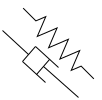
\includegraphics[width=0.3\textwidth]{Deplacement2D-1.png}
    \caption{Floe de glace 2D modélisé par un réseau de ressorts. Le floe est isolé de toutes forces extérieurs. Tous les neouds du réseau ont la même masse $m$, tous les ressorts on la même raideur $k$, et tous les dispositifs visquens ont le même coefficient $\mu$.}
    \label{fig:deplacement2d}
\end{figure}


\noindent Comme nous l'avons présenté aux \cref{eq:F0,eq:e}, le système de la \cref{fig:deplacement2d} est régit par l' équation:
\begin{align} \label{eq:eprime2}
    \forall i \in \mathbb{Z}/3\mathbb{Z}, \quad m \ddot{\bvec{q}}_i = \sum_{j=i+1}^{i+2}C_{ij} \left[  k \left( \Vert \bvec{q}_j - \bvec{q}_i \Vert - L_{ij} \right) \bvec{u}_{ij} - \mu \left\langle \bvec{\dot{q}}_j - \bvec{\dot{q}}_i, \, \bvec{u}_{ij}  \right\rangle  \bvec{u}_{ij}  \right]  , 
\end{align}
où $L_{ij}$ représente la longeur au repos du ressort entre les noeuds $i$ et $j$, et $C_{ij}$ indique si les noeuds $i$ et $j$ sont connectés ou non (pour ce modèle 2D simple, $C_{ij} = 1 \, \forall 0 \leq i,j \leq 2$). Le vecteur unitaire $\bvec{u}_{ij}$ vaut:
$$
\bvec{u}_{ij} = \frac{\bvec{q}_j - \bvec{q}_i}{\Vert \bvec{q}_j - \bvec{q}_i \Vert}.
$$


\paragraph{Simulation par un schéma d'Euler explicite.}

On discrétise par un schéma de différence finies avec $N+1$ pas de temps, et pour une temps de simulations $T$:
$$
\forall i \in \mathbb{Z}/3\mathbb{Z}, \, \forall n \in [\![ 0,N ]\!], \quad  t^n = n\Delta t = n\frac{T}{N}, \quad \bvec{q}_i(t^n) \approx \bvec{q}_i^n.
$$
L'\cref{eq:eprime2} devient:
$$
m\frac{\bvec{q}_{i}^{n+1}-2\bvec{q}_{i}^{n}+\bvec{q}_{i}^{n-1}}{\Delta t^2} = \sum_{j=i+1}^{i+2}C_{ij}\left[ k \left( \Vert \bvec{q}_j^n - \bvec{q}_i^n \Vert - L_{ij} \right) \bvec{u}_{ij} - \mu \left\langle \frac{\bvec{q}_{j}^{n}-\bvec{q}_{j}^{n-1}}{\Delta t} - \frac{\bvec{q}_{i}^{n}-\bvec{q}_{i}^{n-1}}{\Delta t}, \, \bvec{u}_{ij} \right\rangle  \bvec{u}_{ij}  \right],
$$
soit encore:
\begin{align} \label{eq:systeme2D}
    \bvec{q}_{i}^{n+1} = 2\bvec{q}_{i}^{n}-\bvec{q}_{i}^{n-1} + \frac{\Delta t^2}{m} \sum_{j=i+1}^{i+2}C_{ij}\left[ k \left( \Vert \bvec{q}_j^n - \bvec{q}_i^n \Vert - L_{ij} \right) \bvec{u}_{ij} - \frac{\mu}{\Delta t} \left\langle \bvec{q}_{j}^{n}-\bvec{q}_{j}^{n-1} - \bvec{q}_{i}^{n}+\bvec{q}_{i}^{n-1}, \, \bvec{u}_{ij} \right\rangle  \bvec{u}_{ij}  \right].
\end{align}
La simulation de ce modèle par un schéma d'Euler explicite à pas constant sur un intervalle de temps faible ($T = 4$) est présentée à la \cref{fig:PlotDeplacement2D1Conv}, ainsi que les positions des 2 noeuds au début et à la fin de la simulation. La simulation à la \cref{fig:PlotDeplacement2D1NonConv} permet d'observer le problème avec ce schéma ($T = 10$).


\begin{figure}[!h]
    \begin{subfigure}[b]{0.7\textwidth}
        \centering
        \includegraphics[width=\textwidth]{PlotDeplacement2D-1-Conv.png}
        \caption{Simulation des positions des noeuds.}
        \label{fig:dep}
    \end{subfigure}
%     \hfill
    \begin{subfigure}[b]{0.7\textwidth}
        \centering
        \includegraphics[width=\textwidth]{PositionInitFinales.png}
        \caption{Illustration des positions initiales et finales des neouds.}
        \label{fig:pos}
    \end{subfigure}
    \caption{Simulation du système \ref{eq:systeme2D} par un schéma d'Euler explicite avec $T = 4$. La couleurs rouge repésente le noeud $\bvec{q}_1$, le vert le noeud $\bvec{q}_2$, le blue le $\bvec{q}_3$. Les paramètres utilisés ici sont les suivants: $m=6.2$, $k=23.3$, $\mu=3$; à l'instant initiale, les trois noeuds perturbés avec des vitesses d'intensité respectives $v_1=0.3$, $v_2=0.1$, et $v_3=0.1$. Par rapport à l'axe des abcisses, ces vitesses ont sont orintées respectivement de $\theta_1=180^\circ$, $\theta_2=270^\circ$, et $\theta_3=240^\circ$ (voir \texttt{code/simu2D/Deplacement2D-1.ipynb}).}
    \label{fig:PlotDeplacement2D1Conv}
\end{figure}


\begin{figure}[!h]
    \centering
    \includegraphics[width=0.7\textwidth]{PlotDeplacement2D-1-NonConv.png}
    \caption{Simulation du système \ref{eq:systeme2D} par un schéma d'Euler explicite avec $T = 10$. Cette figure utilise les même paramtètres que la \cref{fig:PlotDeplacement2D1Conv}. On observe ici une divergence totale du système.}
    \label{fig:PlotDeplacement2D1NonConv}
\end{figure}

Les \cref{fig:PlotDeplacement2D1Conv,fig:PlotDeplacement2D1NonConv} permettent de constater que le schéma d'Euler explicite (peu importe son pas de temps), n'est pas adapté à ce problème. Nous étudierons donc d'autres alternatives. 

 
\paragraph{Simulation à l'aide des fonction de la librarie Scipy.} À travers ses fonction telle que \texttt{odeint} et $\verb|solve_ivp|$, \texttt{Scipy} offre une solution robuste et élégante pour simuler les systèmes d'ODE de la forme $Y' = AY$.


 




\subsubsection{Modélisation du contact entre deux floes}

Les floes de glace $\Omega_k$ et $\Omega_l$ sont modélisés par des systèmes masse-ressort (à grande raideur). Pour l'instant, nous considérons une moélisation simplifiée qui assimile un floe à un système de (trois) masses reliés par des ressorts (de constante de raideur $k$), et par des dispositifs visqueux de constante $\mu$.
Nous désignerons par $n+1$ le nombre total de noeuds du floe $\Omega_k$, chaque noeud ayant pour masse $m$. De facon similaire, on définit les constantes $k'$, $\mu'$, $n'+1$, $m'+1$ pour le floe $\Omega_l$. Les positions des noeds de $\Omega_k$ seront noté $(q_i)_{0\leq i\leq n}$, tandis que ceux de $\Omega_l$ seront notés $(p_i)_{0 \leq i\leq n'}$ (voir \cref{fig:contactmanuel}). 

\begin{figure}[!h]
    \centering
    \includegraphics[width=0.3\textwidth, angle=-90]{ContactManuel.jpg}
    \caption{Contact entre deux floes aux points $p_0 = q_0$.}
    \label{fig:contactmanuel}
\end{figure}

\noindent On définit la matrice de contact $C$...(voir these Dimitri), et $L_{0j}$.. et $u_{0j}$ ..

\noindent Comme présenté dans les travaux \parencite[p.186]{balasoiu2020halthesis}, le système différentiel qui modélise la percussion s’écrit comme le couplage de deux sous-systèmes. Le premier, dit système intérieur (SI), est à évolution rapide et modélise la propagation des ondes élastiques dans le système masse-ressort. Ici, nous dérivons facilement et réutilisont le SI comme présenté par \citeauthor{balasoiu2020halthesis}. Le second, dit système extérieur (SE), est à évolution lente et modélise la pénétration de l’objet solide dans le système masse-ressorts. Pour dériver le SE sur le floe $\Omega_k$, nous écrivons l'équation de Newton-Euler linéaire\footnote{La rotation du point matériel $q_0$ n'est pas prise en compte ici, d'où l'abscence de l'équation de Newton-Euler angulaire.} au point de contact $q_0$:
\begin{align}  \label{eq:SE}
m \ddot{\bvec{q}}_0 = \bvec{F}_0 + \bvec{F}^c_0 \,,
\end{align}
où 
\begin{align}  \label{eq:F0}
    \bvec{F}_0 = \sum_{j=0}^{n}C_{0j} \left[  \underbrace{k \left( \Vert \bvec{q}_j - \bvec{q}_0 \Vert - L_{0j} \right) \bvec{u}_{0j}}_{\text{Force de rappel}} - \underbrace{\mu \left\langle \bvec{\dot{q}}_j - \bvec{\dot{q}}_0\,, \bvec{u}_{0j}  \right\rangle  \bvec{u}_{0j}}_{\text{Force de dissipation}}  \right] \,,
\end{align}
représente la somme des forces de reaction et de disssipation exercées par le ressort et le dispositif visqueux sur le noeud $q_0$ ; et $\bvec{F}^c_0(t)$ la force de contact durant la collison entre les deux particules. En supposnat qu'il existe un repère de contact $\mathcal{R}^c = \{ q_0, \bvec{n}, \bvec{t} \}$ associé au floe $\Omega_k$ (voir \cref{fig:contactmanuel}), on peut écrire, pour $(\lambda, \beta) \in \Rdeux$ :
\begin{align}  \label{eq:F0c}
    \bvec{F}_0^c = \lambda \bvec{n} + \beta \bvec{t} \,.
\end{align}
Le système intérieur (SE) s'obtient facilement en combinant les équations \cref{eq:SE,eq:F0,eq:F0c}. Le système intérieur (SI) s'obtient lui (pour les autres noeuds du réseau) en y supprimant la force de contact. On obtient au final:
\begin{align} \tag{$E$} \label{eq:e}
\begin{dcases}
    m \ddot{\bvec{q}}_0 = \bvec{F}_0 + \bvec{F}^c_0  \,, &\qquad \text{(SE)} \\
    m \ddot{\bvec{q}}_i = \bvec{F}_i   \,, \quad \quad \quad \forall 1 \leq i \leq n \,. &\qquad \text{(SI)}
\end{dcases}
\end{align}
En ce qui concerne le floe $\Omega_l$, nous procédons de facons similaire et appliqons la 3ème loi de Newton (action-réaction) pour obtenir le système:
\begin{align} \tag{$E'$} \label{eq:eprime}
\begin{dcases}
    m' \ddot{\bvec{p}}_0 = \bvec{F}^{'}_0 - \bvec{F}^c_0  \,, &\qquad \text{(SE)} \\
    m' \ddot{\bvec{p}}_i = \bvec{F}^{'}_i   \,, \quad \quad \quad \forall 1 \leq i \leq n' \,, &\qquad \text{(SI)}
\end{dcases}
\end{align}
où $(\bvec{F}^{'}_i)_{0 \leq i \leq n'}$ sont définis de facon similaire à $\bvec{F}_0$ (voir \cref{eq:F0}):
\begin{align}
    \bvec{F}'_i = \sum_{j=i}^{n'}C_{ij} \left[ k' \left( \Vert \bvec{p}_j - \bvec{p}_i \Vert - L'_{ij} \right) \bvec{u'}_{ij} - \mu' \left\langle \bvec{\dot{p}}_j - \bvec{\dot{p}}_i\,, \bvec{u}'_{ij}  \right\rangle  \bvec{u}'_{ij}  \right] \,.
\end{align}

\noindent Ensuite, on additionne membre à membre les équations des systèmes extérieurs (SE) de \cref{eq:e,eq:eprime} pour éliminer la force de contact. On obtient:
\begin{align}
m \ddot{\bvec{q}}_0 + m' \ddot{\bvec{p}}_0 = \bvec{F}_0 + \bvec{F}^{'}_0 \,.
\end{align}
Remarquons que les positions relatives des noeuds $\bvec{q}_0$ et $\bvec{p}_0$ restent inchangées durant la collision. A l'instant initial, on note donc $\Delta_0 = \bvec{q}_0(0) - \bvec{p}_0(0)$; ainsi : 
\begin{align}
\forall t \in \mathbb{R}^+ \,, \quad \bvec{q}_0(t) - \bvec{p}_0(t) = \Delta_0\,.
\end{align}
Nous avons aisni obtenu les $n+n'+2$ équations nécessaire pour que notre problème de percussion soit bien posé. Elles sont :
\begin{align} \tag{$\mathcal{P}$} \label{eq:problemeP}
\begin{dcases}
    m \ddot{\bvec{q}}_0 + m' \ddot{\bvec{p}}_0 = \bvec{F}_0 + \bvec{F}^{'}_0  \,, &\qquad \text{(SE)} \\
    \bvec{q}_0 - \bvec{p}_0 = \Delta_0 \,, &\qquad \text{(SE)} \\
    m \ddot{\bvec{q}}_i = \bvec{F}_i   \,, \quad \quad \quad \forall 1 \leq i \leq n \,. &\qquad \text{(SI)} \\
    m' \ddot{\bvec{p}}_i = \bvec{F}^{'}_i   \,, \quad \quad \quad \forall 1 \leq i \leq n' \,, &\qquad \text{(SI)}
\end{dcases}
\end{align}

Ensuite, il nous faut introduire des conditions portant sur la conservation de l'énergie, et la condition de non-interpénétration de Signorini\dots







% \section{Les apports du stage}

%\begin{itemize}
%    \item L' utilisation de TIKZ
%\end{itemize}       %% Travaux et apports
% % Chapter 5

\chapter{Déroulement et apports du stage} % 5th chapter title

\label{Chapter5} % For referencing the chapter elsewhere, use \ref{Chapter5} 

%1----------------------------------------------------------------------------------------






\section{Journal de bord}


DONNER AUSSI LES DIFFICULTÉES MAJEURES RENCONTRÉES SEMAINES APRÈS SEMAINES




A LA FIN, FAIRE UN GRAPHIQUE QUI RÉSUME CA


%2----------------------------------------------------------------------------------------






\section{Bilan et future travail}

Durant ce stage, nous avons modéliser et simuler la percussion de floes de glace. Nous avons fait cela en 1 dimension et nous avons convenablement adapté les résultats en simension supérieure, en se servant des travaux précédents sur ce sujet. En plus, nous modélisé et implémenté la fracture en d'un floe de glace 1D. Ceci dit, plusieurs taches restent à effectuer pour porter à fruition notre objectif primaire de creation d'un code de calcul de l’évolution de la banquise à l’échelle des floes de glace:

\begin{itemize}
    \item \textbf{Implémentation de la méthode du champ de phase sue le modèle 1D.} L'approche du champ de phase a longement été présentée à la \cref{subsubsec:approchephase}. Comme nous l'avons indiquée, elle est la mieux adaptée à l'étude de la fracture suivant l'approche variationnel de Francfort et Marigo.
    \item \textbf{Implementation de la fracture au problème 2D.} Durant sa thèse, \citeauthor{balasoiu2020halthesis} a implémenté un modèle quasi-statique de fracture variationnel à travers une méthode éléments finis reposant sur une approche par champ de phase pour régulariser la fracture. Ces travaux sont regroupé dans le dépot sur \texttt{framagit} nommé \href{https://framagit.org/RaK/Griffith}{Griffith}. Il faudra intégré ces travaux au modèle de percussion 2D que nous avons développé durant ce stage.
    \item \textbf{Intégration de la fracture fragile au code de \citeauthor{rabatel2015thesis}.} Comme nous l'avons précisé, \citeauthor{rabatel2015thesis} a, durant sa thèse étudié la dérive d'un ensemble de floes de glace dans la mer. Il faudra donc introduire la fracture de la glace dans ce modèle.
    \item \textbf{Passage en dimension supérieure.} Pour aller plus loin, nous conseillons de passer en trois dimension. Celà dit, les tailles des floes peuvent etre négligeable devant le rayon de la Terre, où la taille de la mer. Il faudra donc prendre celà en considération pour faire des simplifications.
    \item \textbf{Optimiser des codes avec Cython.} En effet, les codes sont écrits en Python durant cette phase . Ce language ne nous permet pour l'instant que d'éfffectuer des simulation avec un nombre restraint de neouds. On pourra donc utiliser \href{https://cython.org/}{Cython} pour faire appel aux fonctions à haute performace du language C. Ou mieux encore, nous pourront reimplémenter tous le code en C$++$ en intégrant les librairies HPC telles que \href{http://www.netlib.org/blas/}{Blas}, \href{https://www.openmp.org/}{OpenMP}, \href{https://developer.nvidia.com/cuda-zone}{CUDA}, etc.
    \item \textbf{Tests de validation en laboratoire.} Des tests en laboratoire sont nécéssaire pour validé les modèles développés. Tout comme \citeauthor{rabatel2015thesis} l'a fait, l'on pourra se servir des données \textbf{ERAinterim} et \textbf{TOPAZ} pour effectuer ces tests.
\end{itemize}






%3----------------------------------------------------------------------------------------




\section{Les apports du stage}


J'ai maitrisé la majeure partie des objectifs que nous nous étions fixés. Cela dit, les apports de ce stages ont été incomptables, et sur plusieurs plans. Tout d'abord sur un plan académique, ou j'ai pris en mains des notions clées des mathématiques appliquées et de l'informatique. Ensuite sur un plan technique, j'ai pu maitriser des outils et faire usage de ressources varirées. Enfin, sur un plan profesionnel ou j'ai pu apprendre d'avantage sur le monde de la recherche.



\subsection{Compétences académique}

\begin{itemize}
    \item \textbf{Simulation de processus physiques:} Ce stage m'a appris à simuler des objects répondant à une loi de comportement bien présice (loi de Newton-Euler, EDO du second ordre) par l'intermédiare de schéma appropriés. Par exmple, un schéma explicite d'ordre 2 pour l'SYSTÈME 2D diverge très fréquement, alors qu'un shéma symplectique (voir \cref{AppendixA}), où un schéma explicite Runge-Kutta d'ordre 4 (RK4) à pas de temps suivant RK5 (comme ceux implémenté par \href{https://docs.scipy.org/doc/scipy/reference/generated/scipy.integrate.solve_ivp.html}{Scipy}) conserve les invariants du système.
    \item \textbf{Prise en main du modèle de rupture de Griffith dans les milieux élastiques:} En lisant les travaux qui ont ptécédé \parencite{balasoiu2020halthesis}, j'ai pu apprendre beacoup sur le modèle de Griffith et la compétition entre les énergie de déformation et de fracture du matériau. J'ai aussi lu les articles \parencite{francfort1998revisiting,bourdin2008variational} et j'ai ainsi assimilé l'approche variationnelle de Francfort, Marigo, Bourdin. Ces notions m'ont poussé à visiter des outils mathématiques très puissant tels que le calcul des variations et la $\Gamma$-convergence (voir \cref{AppendixB}).
    \item \textbf{Maitrise des réseaux de ressorts:} Les travaux de \citeauthor{balasoiu2020halthesis} m'ont également appris comment étudier un matéraux élastiques (réseau de ressorts) par l'intermédiaire d'un processus de poissons \parencite{khasminskii2011stochastic}\footnote{Merci à M. Labbé de m'avoir offert ce livre :)}. J'ai par exmeple appris comment créer (manuellement ou en se servant de la librarie \texttt{Scipy}) un processus de Poinsson répondant à un certain nombre de critères (en particulier l'\emph{intensité}).
    \item \textbf{Développement d'applications en language Python:} Durant ce stage, j'ai énormément améliorer mes compétences en simulation numérique via Python. J'ai par exemple appris comment créer, modifier et déployer un package Python, comment utiliser plusieurs libraries (\texttt{numdifftools}) de calcul scientifique pour mener à bien un projet.
\end{itemize}




\subsection{Compétences techniques}

\begin{itemize}
   \item \textbf{Utilisation de TikZ:} Le premier outils que j'ai maitrisé durant ce stage fut le package LaTex nommé \textt{TikZ}. Sous la recommendation de M. Labbé, je l'ai utilisé au départ comme complémentaire à \href{https://www.diagrams.net/}{diagrams.net}, mais j'ai très vite vu son potentiel et la possibilité de l'utiliser pour virtuellement toutes les dessins.
   \item \textbf{Maitrise de Flask:} \href{https://flask.palletsprojects.com/en/2.0.x/}{Flask} est une micro-framework de développement web en Python. J'ai trouvé que c'est outils permet de construire de belles interface pour effectuer des simulation. Ainsi, l'utilisateur n'a pas besoin d'etre familier avec notre code de calcul pour s'en servir. 
   \item \textbf{Maitrise de Bokeh:} Je me suis très vite rendu compte de la nécéssité de visualiser les résultats. J'ai pris en main la librarie Python \href{https://bokeh.org/}{Bokeh} pour visualiser les déplacements et les vitessess des réseaux de ressorts dans les notebooks interacrifs. 
   \item \textbf{Matrise de Symbolab:} \href{https://www.symbolab.com/}{Symbolab} est un logiciel de calcul symbolique que j'utilise depuis longtemps. Durant ce stage j'ai découvert de nouvelles fonctionnalité et des raccourcis, puis je m'en suis servi surtout pour faire des calculs matriciels en taille élévée ($4\times 4$ par exemple). 
\end{itemize}





\subsection{Compétences professionnnelles}

\begin{itemize}
    \item \textbf{Recherche en milieu professionel:} La première compétence professionnnelle que j'ai gagnée est celle de la recherche dans un milieu aussi prestigieux que le Laboratoire Jacques-Louis Lions. Je n'ai pas manqué d'aide ni de moyens pour effectuer mes taches. J'ai appris à collaborer avec mes pairs et demander de l'aide lorsque nécéssaire. Bien que le LJLL soit un lieu très convivial, la situation sanitaire actuelle m'a ammené à me discipliner pour pouvoir conduire mes travaux de recherche en télétravail.
    \item \textbf{Savoir-faire transfesrables:} A travers ses journées "thé du labo". Ce fut l'occasion de mieux se connaitre et de tisser des liens. Parmis les conpétences transferables que j'ai pu acquerrir durant ce stage, je peux citer l'esprit de recherche, d'entreprise, la gestion du temps, et la collaboration.
\end{itemize}       %% Déroulement du stage
% % Chapter 6

\chapter{Conclusion} % 6th chapter title

\label{Chapter6} % For referencing the chapter elsewhere, use \ref{Chapter6} 

%----------------------------------------------------------------------------------------


Pour conclure, j'ai effectué mon stage de fin d'étude au Laboratoire Jacques-Louis Lions sous la supervision du professeur Stéphane Labbé. Durant six mois au sein de ce célèbre laboratoire de mathématiques appliquées, je me suis confronté au problème de la \emph{fracturation des floes de glace} dans un modèle granulaire. J'ai ainsi pu mettre en pratique mes connaissances en calcul scientifique, en analyse numérique, en EDP, en analyse fonctionnelle, et en développement Python (et bien d'autres) acquises durant ma formation de \href{https://www.unistra.fr/etudes/decouvrir-nos-formations/par-facultes-ecoles-instituts/sciences-technologies/ufr-de-mathematique-et-dinformatique/ufr-de-mathematique-et-dinformatique/cursus/ME195?cHash=3aa4f04702a03e944ed933056abe17f2}{CSMI}. 

À travers les objectifs secondaires que nous nous sommes fixés, j'ai pu comprendre le modèle de rupture de Griffith dans les milieux élastiques en assimilant des domaines clés de l'analyse fonctionnelle tels que la $\Gamma$-convergence, la résonance, et la probabilité; j'ai posé les bases du passage micro/macro du modèle élastique et j'ai développé plusieurs modèles de percussion (1D et 2D). J'ai acquis de l'expérience en programmation d’un modèle mathématique par différents schémas numériques, et en suivi de son intégration à un projet de développement logiciel. Sur un plan technique, j'ai maitrisé plusieurs outils informatiques tels que TikZ, Flask, Bokeh, et Symbolab.

Cela dit, il reste plusieurs travaux à effectuer pour conclure ce travail. Nous pouvons par exemple citer l'implémentation de la méthode du champ de phase dans le modèle 1D, l'implémentation de la fracture dans le problème 2D, le passage en dimension supérieure (2.5D ou 3D), l'optimisation du code, des tests de confirmation de l'approximation par réseaux de ressorts à grande raideur, et des tests de validation des modèles en laboratoire.

Fort de cette expérience et de ses enjeux cruciaux pour l'industrie et pour la planète, j'aimerais apporter ma contribution à la science à travers ce projet et d'autres similaires. Le projet \href{https://sasip-climate.github.io/}{SASIP} qui a fait de la compréhension du \emph{réchauffement climatique en zone polaire} sa mission phare est une initiative à soutenir et à répéter.       %% Conclusion

%----------------------------------------------------------------------------------------
%	THESIS CONTENT - APPENDICES
%----------------------------------------------------------------------------------------

% \appendix % Cue to tell LaTeX that the following "chapters" are Appendices

% Include the appendices of the thesis as separate files from the Appendices folder
% Uncomment the lines as you write the Appendices

% 
% Appendix A

\chapter{Rappels sur les EDO} % Main appendix title
\label{AppendixA}

\section{Le schéma Scymplectique}



EXPLICATION DU MODULE SCIPY INTEGRATE
% 
% Appendix B

\chapter{Le schéma Symplectique} % Appendix B title

EXPLICATION DU MODULE SCIPY INTEGRATE

%\include{Appendices/AppendixC}

%----------------------------------------------------------------------------------------
%	BIBLIOGRAPHY
%----------------------------------------------------------------------------------------

\printbibliography[heading=bibintoc]

%----------------------------------------------------------------------------------------

\end{document}

